\documentclass[review]{elsarticle}
\usepackage[utf8]{inputenc}
\usepackage{graphicx}
\usepackage{amsmath}
\usepackage{caption}
\usepackage{float}
\usepackage{geometry}
\usepackage{booktabs}
\usepackage{siunitx}
\usepackage{pgfplots}
%\usepackage{authblk} % To include affiliations of authors
\usepackage{url}
\usepackage{chemformula} % Formula subscripts using \ch{}
%\usepgfplotslibrary{groupplots}
\pgfplotsset{compat=1.18} % 
\usepackage{xcolor}
\usepackage{comment}
\usepackage{diagbox}
\usepackage{ulem}

\biboptions{sort&compress}

\newcommand{\gc}{\mathrm{g_c}}
\newcommand{\vc}{\mathrm{v_c}}
\newcommand{\ugc}{\mathrm{ug_c}}
\newcommand{\uvc}{\mathrm{uv_c}}

\newcommand{\xca}{-210}
\newcommand{\xcb}{20}
\newcommand{\yc}{140}
\newcommand{\len}{6.5}

\begin{document}
\captionsetup[figure]{labelfont={bf},labelformat={default},labelsep=period,name={Fig.}}

\begin{frontmatter}

\title{\textcolor{red}{Descriptor-Space Mapping of Metal-Organic Frameworks for 
Hydrogen Storage at Room Temperature and Moderate Pressure Using Neural 
Networks} \sout{Inverse Design of Metal-Organic Frameworks for Hydrogen Storage 
at Room Temperature and Moderate Pressure Using Neural Networks}}
\date{}
\author[1]{A. Granja-DelRío \corref{corr}}
\cortext[corr]{Corresponding author}
\ead{alejandra.granja@uva.es}
\author[2]{T. Calonge}
\author[1]{I. Cabria}
\address[1]{Departamento de F\'{\i}sica Te\'orica, At\'omica
y \'Optica, Universidad de Valladolid, ES-47011 Valladolid, Spain}
\address[2]{Departamento de Informática (ATC, CCIA y LSI),
Universidad de Valladolid, ES-47011 Valladolid, Spain}



\begin{abstract}
Metal-Organic Frameworks (MOFs) are promising solid porous materials for 
hydrogen storage at room temperature and low to moderate pressures in Fuel Cell 
Vehicles (FCVs). However, systematic exploration of hydrogen storage 
performance using Grand Canonical Monte Carlo (GCMC), Density Functional Theory 
(DFT), or related methods is computationally expensive. \sout{In this work, an 
Artificial Neural Network (ANN) approach is proposed to accelerate the 
identification of MOFs with favorable hydrogen storage properties.}
\textcolor{red}{This work employs an artificial-neural-network (ANN) surrogate 
to accelerate hydrogen-storage assessment in MOFs via a descriptor-space 
feasibility mapping approach.} The model was trained on a dataset of 
\sout{1000} \textcolor{blue}{5000} MOFs generated from GCMC simulations 
performed at 298.15 K and 25 MPa. Each data sample includes the usable 
gravimetric and volumetric hydrogen storage capacities together with 
\sout{five} \textcolor{blue}{eight} key structural descriptors: porosity, 
framework density, largest pore radius, specific surface area, \sout{and 
specific pore volume} \textcolor{blue}{specific pore volume, degree of 
unsaturation, metal weight percentage and metal atom percentage}. \sout{Unlike 
conventional machine-learning approaches that directly predict hydrogen uptake 
from structural descriptors, the present study formulates the problem from an 
inverse design perspective} \sout{\textcolor{red}{While machine-learning 
surrogates for adsorption in MOFs are widely used for forward property 
prediction and high-throughput screening, the present contribution reframes 
the task as a descriptor-space feasibility mapping of usable gravimetric and 
volumetric capacities at 25~MPa.}} \textcolor{blue}{While machine-learning 
surrogates are used to predict storage capacities from given structures of 
MOFs, the present ANN surrogate identifies regions of the structural-parameter 
space that correspond to MOFs whose storage capacities are equal to or larger 
than the Department Of Energy (DOE) 2025 goals.} \sout{The ANN is used to 
identify regions of the structural-property space compatible with target 
hydrogen storage performances defined by the U.S. Department of Energy (DOE) 
2025 goals.} \sout{This strategy enables rapid screening of candidate MOFs and 
provides physically interpretable guidance to support the targeted design and 
synthesis of materials with enhanced hydrogen storage capacities.} 
\textcolor{blue}{GCMC simulations of a selected group of MOFs with structural 
properties near those identified regions were performed.} \textcolor{red}{A 
pronounced feasibility gap is observed: while a subset of \sout{frameworks} 
\textcolor{blue}{the selected MOFs} approaches the gravimetric target (5.5~wt. 
\%), reaching values up to 11~wt. \%, none in the present dataset meet the 
volumetric requirement (0.040~kg/L) at 25~MPa, with most \sout{candidates} 
\textcolor{blue}{MOFs} falling below 0.024~kg/L. This negative result 
highlights intrinsic trade-offs between porosity and volumetric packing in 
adsorption-based storage at moderate pressure. The resulting descriptor-space 
maps delineate practical boundaries for subsequent simulation or experimental 
screening within the explored feature space.}
\end{abstract}

\end{frontmatter}



%%%%%%%%%%%%%%%%%%%%%%%%%%%%%%%%%%%%%%%%%%%%%%%%%%%%%%%%%%%%%%%%%%%%%%%%%%%%%%%%
\section{Introduction}
%%%%%%%%%%%%%%%%%%%%%%%%%%%%%%%%%%%%%%%%%%%%%%%%%%%%%%%%%%%%%%%%%%%%%%%%%%%%%%%%

Transport is essential for modern life. It connects people and supports trade, culture, and access to basic services. However, it also has strong negative impacts. It is responsible for about 25 \% of greenhouse gas emissions in the EU \cite{zjb+24,cde+22,jena11}, and it increases air and noise pollution as well as habitat loss \cite{tm24,netzeroiea,netzerousa,smcf20,doe25}. For this reason, cleaner energy solutions are needed. 
Hydrogen is seen as a good alternative for reducing emissions \cite{netzeroiea,zjb+24,cstc22,apap19,bw15,bhlk+26,laaz+25}. In vehicles, it can replace fossil fuels, especially in Fuel Cell Vehicles (FCVs). Its gravimetric energy density is very high, 120 MJ/kg, while gasoline offers only 44 MJ/kg \cite{doe25}. However, the volumetric energy density is low at ambient conditions and moderate pressures (0.5-25 MPa). \sout{This makes onboard storage a difficult challenge. Current systems compress hydrogen up to 70 MPa} \cite{atd20,hv14,cwlcz23,rhs+22,breeze18,dy11}\sout{, which is common in commercial compressed-gas storage technologies, but increases cost, system complexity, and safety requirements.}

\textcolor{red}{Hydrogen storage can be achieved using several technological routes, including high-pressure compression, cryogenic liquefaction, and adsorption-based mechanisms such as physisorption. Compression and liquefaction are technologically mature but involve substantial energetic penalties, elevated costs, and demanding safety and maintenance requirements \cite{cwlcz23,bww+21,breeze18,hv14,atd20,rhs+22,h2tanks,llk+22,zuttel03}}. Current systems compress hydrogen up to 70 MPa \cite{atd20,hv14,cwlcz23,rhs+22,breeze18,dy11}, which is common in commercial compressed-gas storage technologies, but increases cost, system complexity, and safety requirements. To face this problem, the US Department of Energy (DOE) defined targets for 2025. They require at least 5.5 wt. \% for the usable gravimetric capacity, $\ugc$, and 0.040 kg/L for the usable volumetric capacity, $\uvc$ \cite{doe25,ahg+18}. These values are considered essential for real applications, where driving ranges above 600 km are needed \cite{cwlcz23,bww+21,breeze18,hv14,dy11}.

\textcolor{red}{These targets are system-level metrics defined for the complete storage system (tank, media, and balance-of-plant) under the DOE ``usable'' convention, which denotes the hydrogen that can be reversibly stored and delivered between specified operating pressures and temperatures \cite{usdrivetarget2017,usdrivetarget17,doetables17,doe25}. As such, they implicitly reflect tank geometry, maximum pressure, thermal management, and packaging constraints, and are commonly employed in system-level trade studies \cite{ahluwalia24,hsecoe19}.}



\textcolor{red}{
Among alternative storage routes, adsorption-based systems-often referred to as adsorbed hydrogen gas (AHG) concepts-have attracted increasing attention as potential complements to high-pressure compressed hydrogen storage. By exploiting physisorption in porous materials, these systems aim to operate at comparatively moderate pressures and near-ambient temperatures. System-level analyses suggest that such operation may reduce compression energy requirements, improve safety margins, and simplify thermal management, although typically at the expense of increased storage volume \cite{zuttel03,ahp12}. From a materials perspective, however, achieving sufficiently high gravimetric and especially volumetric storage densities under these milder operating conditions remains a major scientific and engineering challenge \cite{jbpr23,nasm22,zwy+22,fvy+22,Li22,sap+21,jje+21,ykc+18,wcd+18,yck+17,bd15,ahluwalia24,hsecoe19,doerecord25}.
}

\textcolor{red}{Porous crystalline materials, particularly Metal–Organic Frameworks (MOFs), have therefore attracted growing interest as candidates for adsorption-based hydrogen storage. Their modular architectures, wide tunability of pore size and chemistry, and exceptionally high specific surface areas offer unique opportunities to balance porosity and framework density in pursuit of improved storage performance \cite{dbc22,fgf22,gsi+18,jbpr23,nasm22,zwy+22,fvy+22,Li22}. By judicious selection of metal nodes and organic linkers, MOFs can be tailored to enhance hydrogen–framework interactions while preserving accessible pore volume.}

\textcolor{red}{The hydrogen adsorption behavior of MOFs has been extensively investigated using complementary experimental and computational strategies. Experimental studies have characterized adsorption isotherms and thermodynamic properties under a range of conditions \cite{hwl+23,pam23,smb+23,zzh23,lly+22}, while molecular simulations have played a central role in screening large materials sets and interpreting adsorption mechanisms \cite{ssc23,zzh23}. Among simulation techniques, the Grand Canonical Monte Carlo (GCMC) method is particularly well established for modeling gas adsorption in porous solids, providing quantitative predictions of hydrogen uptake as a function of pressure and temperature \cite{cabria24,zzh23,gc24,cc22}.}

\sout{Among possible storage materials, Metal-Organic Frameworks (MOFs) are very promising. They combine high surface area, tunable pore sizes, and flexible design. This makes them good candidates for hydrogen storage near room temperature through physisorption \cite{gc24}.}

\textcolor{red}{
Extensive experimental and computational studies indicate that deliverable 
hydrogen in MOFs at near‑ambient temperature depends jointly on metal nodes, 
linker chemistry, and pore topology. Light metal centers and open metal sites 
(OMS) tend to increase adsorption enthalpy and usable working capacity; 
aromatic, rigid linkers support high specific surface areas; and interconnected 
cage/channel topologies favor deliverable capacity when densification is 
feasible \cite{smh24,alp+17}. Representative systems illustrate these trends: 
Mg/Co/Ni–MOF‑74 \cite{kjsk+24} variants leverage OMS to raise near‑ambient 
uptake; HKUST‑1 (Cu-BTC) \cite{morb+22} benefits from porosity and can achieve 
high volumetric capacity upon monolithic densification; UiO‑66\cite{ltjw+25} 
provides robustness from Zr nodes; and IRMOF families maximize surface area 
with aromatic linkers \cite{ksaa+23}. In addition, compositional and 
topological guidelines emerging from prior studies suggest that light metals 
(e.g., Mg, Al) lower framework density and often favor gravimetric metrics; 
transition‑metal OMS (e.g., Co, Ni) raise adsorption enthalpy at 298~K; and 
Zn/Al frameworks constructed with rigid aromatic linkers can achieve high 
specific surface areas, but may require densification to approach volumetric 
targets \cite{smh24,alp+17,morb+22}.}

\textcolor{red}{These literature-derived trends are used to motivate the 
selected geometric descriptors and to interpret the descriptor-space regions 
identified by the ANN throughout the Results. In particular, the observed 
feasibility regions are discussed in light of metal-node effects, linker 
rigidity, and pore topology reported in prior studies.} Still, finding new MOFs 
that meet both gravimetric and volumetric targets is not straightforward. It 
often requires extensive experimental work or computationally demanding 
simulations such as Grand Canonical Monte Carlo (GCMC) and Density Functional 
Theory (DFT) \cite{ltc24,cltgv21}. 

\textcolor{red}{To mitigate the computational expense of large-scale GCMC/DFT 
studies,} in recent years, ML techniques have been extensively applied to 
accelerate the prediction of hydrogen storage properties in MOFs and other 
porous materials \textcolor{red}{\cite{bdci+18,wfzz+24,sg20,ylbt+25}}. Previous 
studies have explored the use of \sout{ANN like random forests} 
\textcolor{red}{Machine-learning models such as artificial neural networks, 
random forests, kernel-based regressors, and other supervised learning 
approaches \cite{moc23,ofcg+24}} to predict hydrogen uptake or deliverable 
capacities from structural descriptors \cite{wwyq25,cbc+25,qxx+24,sra23,gm21,
as21,aaps25,sc24}. \sout{These approaches have demonstrated that data-driven 
models can significantly reduce the computational cost associated with 
high-throughput GCMC or DFT simulations.}

\textcolor{red}{In porous-materials screening, ML surrogates trained on GCMC 
have enabled large‑scale assessments of MOFs and related frameworks; 
active‑learning strategies further reduce simulation budgets and help navigate 
composition–structure spaces \cite{adpw+19,gsi+18,moc23,ofcg+24,bdci+18,
wfzz+24,sg20,klk20,sc24,klaf+25}. Most reported workflows target forward 
prediction \textcolor{blue}{of properties}, whereas the present study adopts 
an inverse mapping view-inferring 
feasible descriptor regions that satisfy DOE usable‑capacity thresholds at 
298~K and 25~MPa.}
 
\sout{However, most existing studies focus on the direct prediction of hydrogen 
storage performance from known structural features, effectively addressing a 
forward-design problem.} In contrast, less attention has been paid to the 
\sout{inverse formulation} \textcolor{red}{inverse mapping formulation}, where 
desired storage targets are used to infer regions of the structural-property 
space that could host suitable materials. This limitation restricts the direct 
applicability of ML models as design-guidance tools for experimental synthesis. 
\textcolor{red}{In this context, the term ``inverse'' refers to the inference 
of feasible ranges of structural descriptors consistent with target performance 
metrics, rather than to the direct generation or chemical design of new MOF 
structures.}
\sout{Tens of thousands of synthesized MOFs and millions of theoretical and not synthesized MOFs have been reported} %\cite{llk+22,spst21}.}
\sout{Their large diversity and the use of different metals give researchers many options to design new structures with high potential for hydrogen storage.}
\sout{From a computational perspective, the identification of suitable MOFs for onboard hydrogen storage can be formulated as a search problem within a high-dimensional materials space.}
\sout{To do that, a MOFs table will be available.}
\sout{Each row will store the characteristic parameters of a given material.}
\sout{The mentioned GCMC will provide the corresponding $\uvc$ and $\ugc$, as it will be described in the following section.}
\sout{All this information will make up the dataset for any ML algorithm, in this work, used as regression method.}
\sout{AMETODOLOGIA, also know as function estimator \cite{geron2019}.}
\sout{AMETODOLOGIA Several ML function estimators have been tested and discarded such as decision tree or support vector machine methods and finally, a method based on ANN was selected and will be presented.} \textcolor{red}{
From a data-driven perspective, the identification of suitable MOFs for onboard 
hydrogen storage can be formulated as a regression problem linking structural 
descriptors to usable storage capacities. Machine-learning models can then be 
used as surrogate representations of this relationship, enabling efficient 
exploration of the materials space \cite{pkkl+24}.
}

The ANN will be trained using a dataset composed by the usable storage 
capacities at 298.15 K and 25 MPa plus \sout{five} \textcolor{blue}{eight} 
structural properties of \textcolor{blue}{5000} \sout{1000} MOFs. 
\textcolor{red}{The \textcolor{blue}{5000} \sout{1000} MOFs used in this 
work were selected from the 
Cambridge Crystallographic Data Centre (CCDC) database \cite{ccdc,mlwt+17}, 
which contains experimentally synthesized and structurally resolved MOFs. 
Therefore, the dataset is composed of real materials with experimentally 
reported crystal structures, rather than hypothetical or computationally 
generated frameworks.} The usable capacities were obtained by means of GCMC 
simulations performed using an in-house code published in GitHub \cite{mcmgs}. 
When ANNs are applied in the field of materials science, the usual procedure is 
as follows: the structural parameters of the materials are the inputs and the 
desired capabilities of the materials are the outputs.  In this work, an 
alternative strategy is explored, for given $\ugc$ and $\uvc$ (given/desired 
properties), \sout{the ANN estimates the ranges of \sout{five} 
\textcolor{blue}{eight} structural parameters 
of a hypothetical MOF whose usable storage capacities will be equal or larger 
than the DOE capacity targets for 2025} \textcolor{red}{the ANN estimates 
feasible ranges of \sout{five} \textcolor{blue}{eight} structural descriptors 
associated with storage 
capacities approaching or exceeding the DOE 2025 usable targets within the 
surrogate model.} Finally, GCMC simulations of MOFs whose structural properties 
are close to the structural properties predicted by the ANN, will be also 
performed and analyzed. 
 
\sout{The main novelty of the present work lies in formulating hydrogen storage 
optimization in MOFs as an inverse-design problem at near-ambient temperature 
and moderate pressure.} \textcolor{red}{The present work explores the use of an 
inverse surrogate mapping in descriptor space to assist MOF hydrogen-storage 
screening at near-ambient temperature and moderate pressure, framed by DOE 
usable \textcolor{blue}{hydrogen storage capacity} targets.} Instead of predicting storage capacities from given 
structures, the ANN is used to identify regions of the structural-parameter 
space that are consistent with DOE performance targets. \textcolor{red}{Rather 
than claiming direct material design, the present work positions the ANN as a 
feasibility-mapping tool that delineates regions of structural-parameter space 
compatible with DOE targets, thereby complementing existing high-throughput 
screening and simulation-based approaches.} \textcolor{red}{\sout{We also 
clarify the scope and limitations of the present model:} \textcolor{blue}{The 
scope and limitations of the present model are also clarified:} the ANN is not 
intended to capture detailed chemistry-dependent binding physics, but rather to 
identify feasible regions of descriptor space consistent with system-level 
performance targets. This limitation is explicitly stated to avoid 
over-interpretation of the results.}

\sout{This shift from forward prediction to inverse mapping provides actionable 
guidance for materials design and complements existing high-throughput 
screening methodologies.} \textcolor{red}{This inverse formulation provides 
qualitative guidance for narrowing the descriptor space of \sout{candidate 
materials} \textcolor{blue}{MOFs} and complements established high-throughput 
simulation workflows.} The present work builds upon previous data-driven 
studies while explicitly positioning the ANN as a complementary tool to 
conventional high-throughput screening approaches rather than as a replacement 
for detailed molecular simulations. 



%%%%%%%%%%%%%%%%%%%%%%%%%%%%%%%%%%%%%%%%%%%%%%%%%%%%%%%%%%%%%%%%%%%%%%%%%%%%%%%%
\section{Methodology}
%%%%%%%%%%%%%%%%%%%%%%%%%%%%%%%%%%%%%%%%%%%%%%%%%%%%%%%%%%%%%%%%%%%%%%%%%%%%%%%%

%%%%%%%%%%%%%%%%%%%%%%%%%%%%%%%%%%%%%%%%%%%%%%%%%%%%%%%%%%%%%%%%%%%%%%%%%%%%%%%%
\subsection{Grand Canonical Monte Carlo Simulations}
%%%%%%%%%%%%%%%%%%%%%%%%%%%%%%%%%%%%%%%%%%%%%%%%%%%%%%%%%%%%%%%%%%%%%%%%%%%%%%%%

Grand Canonical Monte Carlo (GCMC) simulations were performed to evaluate 
the total and usable hydrogen gravimetric and volumetric storage capacities 
of MOFs chosen from the Cambridge Crystallographic Database Centre (CCDC) 
\cite{ccdc}. The simulations were carried out at 298.15 K with pressures at 
0.5 and 25 MPa. Each GCMC run consisted of \sout{ten} \textcolor{blue}{one} 
million steps. The first \sout{five} \textcolor{blue}{half a} million were 
used to reach equilibrium, and the last 
\sout{five} \textcolor{blue}{half a} million 
were employed to calculate the storage values. The Metropolis algorithm was 
applied during all iterations \cite{metropolis87}. The types of moves on 
each iteration were assigned with the following probabilities, after running 
some tests: 20 \% for molecular displacement, 40 \% for deletion, and 40 \% 
for insertion \cite{cc22,gc24,gc24a}. The chemical potential was determined 
with the Soave-Redlich-Kwong (SRK) equation of state \cite{soave72}. The 
values for the acentric factor $\omega$, the critical pressure $P_c$, and 
the critical temperature $T_c$ of hydrogen \sout{was} \textcolor{blue}{were} 
taken from Zhou and Zhou \cite{zz01} and Xu et al. \cite{xdy12}. 
 
The interactions between the framework atoms and the gas molecules were 
described with Lennard-Jones (LJ) potentials \cite{lennard24}. The LJ 
parameters were calculated using the Good-Hope combining rule for $\sigma$ 
\cite{gh70} and the Berthelot rule for $\epsilon$ \cite{berthelot1898}. 
Specific LJ parameters were used for the C and \ch{H2} interaction, without 
applying the Berthelot-Good Hope combining rule. \textcolor{red}{No partial 
charges were assigned to the framework atoms, consistent with 
previous studies showing that van der Waals interactions dominate hydrogen 
adsorption at 298~K and moderate pressures. While this LJ-only treatment is 
common for room‑temperature\ch{H2} adsorption, it does not explicitly capture 
chemistry‑dependent effects such as open metal sites, polarization, or 
functional-group contributions. As a result, the GCMC predictions and therefore 
the ANN surrogate trained on them, inherit the limitations of this force field 
choice, which should be considered when interpreting the feasibility maps.}
The values of the LJ 
parameters of the atoms and molecules used in the simulations can be found in 
GitHub \cite{mcmgs}. The cutoff radius was set to 20 \AA{}, after running 
several tests \cite{cc22,gc24,gc24a}. In the GCMC simulations, the atoms that 
composed the MOFs were treated as rigid. 

The input of the program for each MOF consisted mainly on the cell of the 
MOF, obtained from the CIF (Crystallographic Information File) file on the 
CCDC database. Part of the input was also the number of iterations, the 
probabilities of the types of moves, the type of equation state (SRK in the 
present case) and the cutoff radius. The program calculates the total and 
usable volumetric and gravimetric storage capacities, which are defined in 
the next paragraphs. \textcolor{red}{All \textcolor{blue}{5000} \sout{1000} structures used in this study 
correspond to experimentally reported MOFs deposited in the CCDC. No hypothetical or algorithmically generated frameworks were included. This ensures that the surrogate model is trained exclusively on realistic geometries derived from experimentally characterized materials.
These GCMC-derived capacities serve as the target variables for the subsequent surrogate modeling. The ANN does not generate new structures but maps relationships between descriptor ranges and storage metrics within the explored dataset.
}
 
Prior to the GCMC simulations, all MOF structures obtained from the CCDC were carefully prepared for computational use. 
\sout{Solvent molecules and non-framework species were removed from the CIF files, and the structural integrity of the frameworks was verified by checking atomic positions and unit cell parameters. As a result, all structures used in this work are computation-ready and equivalent in quality to those provided by curated databases such as the CoRE MOF database.}
\textcolor{red}{Solvent molecules and guest species were removed from the CIF files, and structural integrity was checked by verifying atomic positions, bonding, and unit-cell consistency. This manual cleaning step ensures that all structures are solvent-free and suitable for adsorption simulations. Although the dataset is not directly taken from the CoRE MOF database, the preparation procedure follows the same principles used to generate computation‑ready MOF structures (i.e., removal of disordered solvents, resolution of partial occupancies, and validation of cell geometry).}
 
\sout{The five} \textcolor{blue}{Five of the} structural parameters of each MOF 
were obtained by means of the Zeo++ code \cite{zeoplusplus}. Those parameters 
were: the density in kg/L, the porosity (a dimensionless magnitude; its values 
are between 0 and 1), the radius of the largest pore of the MOF, $R_i$, in 
\AA{}, the specific surface area, SSA, in m$^2$/g, and the specific pore 
volume, SPV, in cm$^3$/g. \textcolor{blue}{The degree of unsaturation, the 
metal weight percentage and the metal atom percentage of the MOF were 
calculated by the mcmgs code \cite{mcmgs}.} \textcolor{red}{These \sout{five} 
\textcolor{blue}{eight} descriptors primarily capture geometric and textural 
properties of the frameworks. Chemistry-dependent effects such as specific open 
metal sites, framework polarization, functional group chemistry, or catenation 
are not explicitly \textcolor{blue}{, but indirectly} encoded in this 
descriptor set \textcolor{blue}{, through the degree of unsaturation, the
metal weight percentage and the metal atom percentage}. Consequently, the 
descriptor-space feasibility maps produced here should be interpreted as 
geometric feasibility regions within the explored feature space, rather than as 
complete predictors of chemistry‑specific adsorption behavior.
}



%%%%%%%%%%%%%%%%%%%%%%%%%%%%%%%%%%%%%%%%%%%%%%%%%%%%%%%%%%%%%%%%%%%%%%%%%%%%%%%%
\subsubsection{Definitions of Storage Capacities}
%%%%%%%%%%%%%%%%%%%%%%%%%%%%%%%%%%%%%%%%%%%%%%%%%%%%%%%%%%%%%%%%%%%%%%%%%%%%%%%%

In these simulations, the total volumetric storage capacity of hydrogen gas at 
pressure $P$ and temperature $T$, $\vc(P,T)$, also referred to as the density 
of stored gas, is expressed as

\begin{equation}
\label{vc}
\vc(P,T) = \frac{M_g(P,T)}{V} \;,
\end{equation}

\noindent
where $M_g(P,T)$ corresponds to the total mass of gas (hydrogen) stored inside 
the simulation box at pressure $P$ and temperature $T$, and $V$ denotes the box 
volume. In this work, $\vc$ is reported in units of kg of \ch{H2}/L.

The total gravimetric storage capacity at pressure $P$ and temperature $T$, 
$\gc$$(P,T)$, is determined from

\begin{equation}
\label{gc}
\gc(P,T) = \frac{100 M_g(P,T)}{M_g(P,T) + M_{ads}} \;,
\end{equation}

\noindent
with $M_{ads}$ represents the mass of the porous adsorbent material contained 
in the simulation cell, respectively. The total $\gc$ is expressed in weight 
percent (wt. \%).

The usable gravimetric ($\ugc$) and volumetric ($\uvc$) capacities are 
calculated based on the mass of adsorbed hydrogen and the framework only, 
following DOE conventions. The total system mass, including tanks or supports, 
is not included in these calculations.  The usable gas mass at $P$ and $T$, 
$M_{ug}(P,T)$, is defined as the difference between the total gas mass stored 
at a given pressure $P$ and temperature $T$ and the gas mass that remains at 
the lower (depletion) pressure, $P_{dep}$, at the same $T$, $M_{ug}(P,T)$ 
= $M_g(P,T) - M_g(P_{dep},T)$.  In this work, the depletion pressure was 
set to $P_{dep} = 0.5$ MPa, consistent with values used in the literature 
for defining usable or working hydrogen storage capacities in adsorption 
systems. This choice corresponds to the lower bound of pressures accessible 
in typical fuel cell operation \cite{cltgv21,rscf22}.  The usable volumetric 
and gravimetric capacities, also called working or deliverable capacities 
\cite{doe25,ahg+18,sh16}, follow directly from Eqs.~\ref{vc} and~\ref{gc}, 
respectively, replacing the total mass, $M_g(P,T)$, by the usable mass, 
$M_{ug}(P,T)$, into the definitions. The usable and total capacities have the 
same corresponding units: gravimetric in wt. \% and volumetric in kg/L. In 
this study, only the usable storage capacities are considered and discussed. 


%%%%%%%%%%%%%%%%%%%%%%%%%%%%%%%%%%%%%%%%%%%%%%%%%%%%%%%%%%%%%%%%%%%%%%%%%%%%%%%%
\subsection{Dataset}
%%%%%%%%%%%%%%%%%%%%%%%%%%%%%%%%%%%%%%%%%%%%%%%%%%%%%%%%%%%%%%%%%%%%%%%%%%%%%%%%

Several ML methods were considered and implemented using a dataset of \sout{1000} 
\textcolor{blue}{5000}  
MOFs, which was structured as a table with \sout{seven columns and 1000 rows.}
\textcolor{blue}{ten columns and 5000 rows.} Each 
row represents one MOF and contains: the two usable capacities ($\ugc$ in wt. 
\% and $\uvc$ in kg/L at 298.15 K and 25 MPa) and the \sout{five} 
\textcolor{blue}{eight} basic structural 
parameters. The usable capacities were obtained from GCMC simulations at 0.5 
MPa and 25 MPa performed on MOFs randomly selected from the CCDC database. In 
this work, the ANN takes the two usable capacities as inputs and predicts the 
\sout{five} \textcolor{blue}{eight} structural magnitudes as outputs. 



%%%%%%%%%%%%%%%%%%%%%%%%%%%%%%%%%%%%%%%%%%%%%%%%%%%%%%%%%%%%%%%%%%%%%%%%%%%%%%%%
\subsection{Machine Learning Regression \label{subsec:MLR}}
%%%%%%%%%%%%%%%%%%%%%%%%%%%%%%%%%%%%%%%%%%%%%%%%%%%%%%%%%%%%%%%%%%%%%%%%%%%%%%%%

ML Theory originally formulated two fundamental supervised learning challenges: classification and regression \cite{hastie2009elements, bishop2006}.  From an external data point of view, the difference between them lies simply in the numerical type of the desired output associated with each input. In effect, for classification problems, the output needs to be discrete while for regression, it must be continuous \cite{mitchell97}. From decision trees up to some of approaches belonging to the large group called ``Linear Methods'' have both classification and regression version. \sout{Without a doubt, the} \textcolor{blue}{The} most relevant examples for that application are in the ANN category, since they could simulated a wide variety of functions even if a high no linearity will be present \cite{witten2011data}. Before model training, an experimental protocol and evaluation metric were defined. A Hold-Out strategy with a 2/3-1/3 split between training and testing sets was adopted as an initial validation procedure \cite{hastie2009elements}. The coefficient of determination, R$^2$, was selected as the primary regression metric, as it provides a direct measure of the proportion of variance explained by the model \cite{james2021}.

In order to define an appropriate regression framework for the present problem, several widely used supervised learning regressors were considered, following standard practice in the scientific literature \cite{witten2011data}:
\begin{itemize}
    \item Decision Tree Regressor (DTR)
    \item Support Vector Machine with a gaussian kernel (SVR)
    \item Multilayer Perceptron Regressor (MLP-R)
\end{itemize}

The first two regressors were programmed in Python using the scikit-learn 
module. Due to their implementation requirements, it was necessary to handle 
a list of individual regressor: one for each output. Each list of these ML 
regressor was integrated into a single object, for which the typical methods 
(\_\_init\_\_, fit, predict, and score) were implemented. Respect to the last 
method, MLP-R, it was opted for direct PyTorch implementation rather than using 
the corresponding scikit-learn module. This decision was driven by PyTorch's 
superior flexibility, which allowed us to experiment with different activation 
functions across distinct layers \cite{rpn20} and also because MLP yields 
robust and reliable results as a nonlinear regressor \cite{goodfellow2016deep}. 
 
 

%%%%%%%%%%%%%%%%%%%%%%%%%%%%%%%%%%%%%%%%%%%%%%%%%%%%%%%%%%%%%%%%%%%%%%%%%%%%%%%%
\subsection{Multilayer Perceptron Regressor}
%%%%%%%%%%%%%%%%%%%%%%%%%%%%%%%%%%%%%%%%%%%%%%%%%%%%%%%%%%%%%%%%%%%%%%%%%%%%%%%%

Following the MLP architecture, an artificial neural network is proposed as the final method. As it can be seen in Fig.~\ref{regressor}, the model has the same size (ten neurons) for the hidden layers. The number of nodes for the rest of layers are adjusted according to the input and output vectors dimensions. Respect to the activation functions for each layer, it is necessary to take in mind that it is a regression problem, which implies to use the identity as activation function in the output. For the hidden layers, an activation function is needed to be chosen. That function must be restricted to be continuous, bounded and monotonically  increasing, in order to maintain the numerical stability of the system \cite{haykin1999neural}. In addition, because the training algorithm is based on the gradient operation, this activation function has to be differentiable. Finally, the parameters calculated by the model correspond to physical magnitudes that does not admit negative or null values. For all these reasons, the choice of the activation function will be the sigmoid, also known as logistic function \cite{bishop1995mlp}.

\begin{figure}[ht]
    \centering
    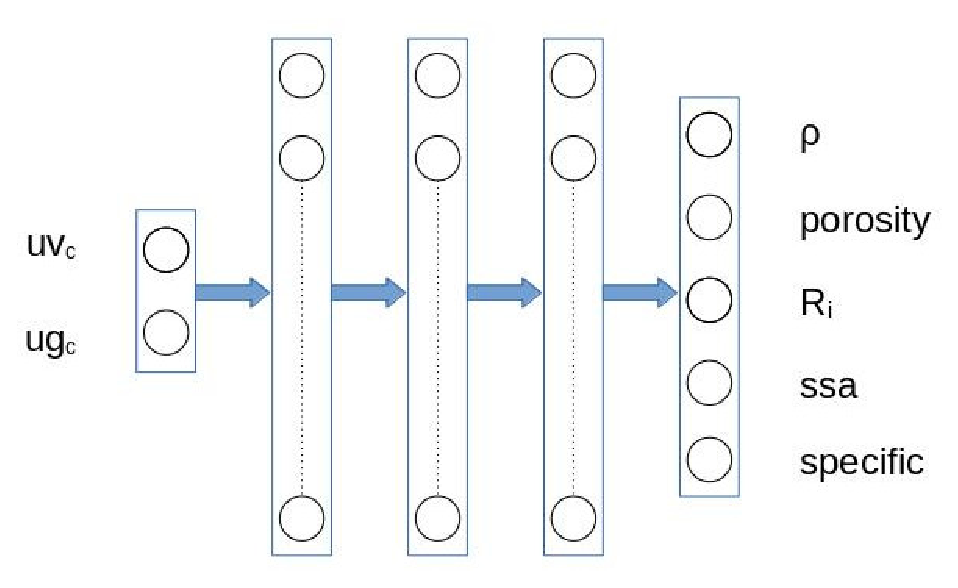
\includegraphics[width=0.75\linewidth]{Arquitectura-MLP-Recortado.eps}
    \caption{MLP Regressor Architecture}
    \label{regressor}
\end{figure}


After the hyperparameter exploration stage, the selected MLP architecture is retrained using the full dataset. In this final training step, all available samples are combined to build a single regression model, ensuring that the maximum amount of information is used. This procedure is standard practice once model configuration has been fixed, and it avoids unnecessary loss of training data due to validation splits.

The rest of implementation details correspond to computation topics. First of all is the programming language and the interactive development environment (IDE). In this particular case, both Python and Jupyter were chosen. However, the most relevant tool for the ANN was PyTorch \cite{pytorch}, which has been built upon tensor calculus to enable an efficient and flexible Deep Learning computation. All the proposed model programs were prepared to be executed automatically on both CPU and GPU; the last option only works if a corresponding hardware device is available and compatible with the CUDA\footnote{Compute Unified Device Architecture - NVIDIA's parallel computing platform and programming model.}or ROCm\footnote{ROCm: AMD's open-source alternative to NVIDIA's CUDA.} version used by PyTorch. Under this configuration, the ANN must optimize a total of 305 trainable parameters. Given the availability of 900 training samples-corresponding to 9 out of the 10 cross-validation folds (see the following paragraph)-and considering that each sample contains \sout{five} \textcolor{blue}{eight} attributes, the risk of undertraining is effectively mitigated. Specifically, the ratio of inputs per weight (equal to 6) is sufficiently high to ensure adequate learning \cite{vapnik1999nature}.

%Note: The ratio of inputs per weight is 6?
%Note: The ratio of inputs per weight is sufficiently high?

Regarding the experimental methodology, Cross-Validation was chosen instead of 
the Hold-Out method used in the preceding subsection. Hold-Out was adequate 
there because only a single numerical value was required for preliminary 
comparison and model screening. However, to draw reliable conclusions, 
a single Hold-Out split is insufficient; multiple experiments with varying 
train/test splits are necessary. Repeated Hold-Out could be a viable solution, 
as the variance of the estimate does not depend on a single split but is 
distributed across multiple experiments. Cross-Validation offers a similar 
advantage but with a key benefit: it ensures that all samples are used for 
both training and testing. This property cannot be guaranteed by Repeated 
Hold-Out \cite{james2021}. 

Previously, each input and output was scaled into the interval [0,1]. In this step, there is only one thing left to do with samples: organizing them into batches. With the aim to avoid any rote learning, the samples will be permuted in each epoch. As it is well known, this task is the foundation for every Stochastic Optimization process, that will also improve the power of generalization, which is the main goal of any machine learning method \cite{bottou2018optimization}.

To execute the algorithm, it is necessary to set some optimization issues. The most important is the cost function. In a regression problem, the Mean Squared Error (MSE) is a very good candidate for assessing optimization and performance \cite{bishop2006}. The next step consists on the optimizer election according to the preceding lost function. The Adaptive Moment Estimation (ADAM) is probably the most popular ANN optimizer \cite{choi2020survey}. It is based on gradients that include not just the momentum term in an adaptive manner, but also incorporates several regularization algorithms like L1 and L2 \cite{kingma2015adam}.

The model implementation was split into two phases:
\begin{itemize}
    \item Hyperparameters setting
    \item Production mode
\end{itemize}

The first phase requires extensive trial-and-error experimentation, guided by empirical rules, to identify suitable MLP hidden layer architectures and optimizer hyperparameters (e.g., learning rate, momentum, and regularization coefficients). This represents the most computationally expensive phase, as the number of trials is multiplied by the number of cross-validation folds (10).

%Regarding the computational effort required to train the proposed ANN, the elapsed time for 200 epochs of the first system was less than three minutes on a Linux virtual machine with eight cores of an Intel(R) Xeon(R) Gold 6128 CPU @ 3.40 GHz. It shows that a GPU is not crucial for the present work.



%%%%%%%%%%%%%%%%%%%%%%%%%%%%%%%%%%%%%%%%%%%%%%%%%%%%%%%%%%%%%%%%%%%%%%%%%%%%%%%%
\section{Results and Discussion}
%%%%%%%%%%%%%%%%%%%%%%%%%%%%%%%%%%%%%%%%%%%%%%%%%%%%%%%%%%%%%%%%%%%%%%%%%%%%%%%%

The ML regressors (DTR, SVR and MLP-R) were applied to the MOFs dataset. The 
results are shown and compared in Table~\ref{tab:placeholder}. Only the 
coefficient of determination (R$^2$) values obtained for the test dataset are 
shown, as this is the most important metric in the ML environment, given its 
direct relationship to the generalization power of the ML methods 
\cite{goodfellow2016deep}.

\begin{table}[H]
    \centering
    \begin{tabular}{|c|c|c|c|}\hline
         ML regressor:&  DTR&     SVR&     MLP-R\\\hline
         R$^2$&          0.8234&  0.5495&  0.8723\\\hline
    \end{tabular}
    \caption{R² comparison for several ML regressors}
    \label{tab:placeholder}
\end{table}

Consequently, based on Table \ref{tab:placeholder}, the method chosen for the 
final implementation is MLP-R. As with the previous two ML regressors or 
methods, a corresponding object with the typical PyTorch ``\_\_init\_\_ '' and 
``forward'' methods has also been created (detailed in the next section). At a 
more abstract level, the \sout{five} \textcolor{blue}{eight} outputs are not 
independent; instead, they are integrated into a single MLP. This enables the 
modeling of potential cross‑dependencies among output variables, which the two 
previous ML methods ignore. To further assess the robustness and stability of the selected MLP-R, a 10-fold 
cross-validation procedure was performed. Each fold contained \sout{900} 
\textcolor{blue}{4500} data points for training and \sout{100} 
\textcolor{blue}{500} for testing. Table \ref{tab:CV-MLP-R} summarizes the 
results from the best-tested hyperparameter set.

\begin{table}
    \centering
    \begin{tabular}{lrccc}\toprule
 FOLD (CV)& MSE (train)& MSE (test)& R$^2$ (train)&R$^2$ (test)\\\midrule
          0&0.002066&  0.002056&  0.885354&  0.898407\\
          1&0.002214&  0.002417&  0.858594&  0.844268\\
          2&0.002134&  0.003154&  0.883937&  0.878659\\
          3&0.002033&  0.001567&  0.898638&  0.875035\\
          4&0.002206&  0.001871&  0.856156&  0.837287\\
          5&0.001999&  0.001691&  0.910156&  0.909507\\
          6&0.002044&  0.002102&  0.893892&  0.893620\\
          7&0.001790&  0.003677&  0.886273&  0.858905\\
          8&0.001878&  0.002324&  0.870179&  0.879475\\
          9&0.002053&  0.001649&  0.859180&  0.854832\\
 \textbf{Average}& \textbf{0.002042}& \textbf{0.002251}& \textbf{0.880236}&\textbf{0.872999}\\ \bottomrule
    \end{tabular}
    \caption{Cross Validation MLP-R Results}
    \label{tab:CV-MLP-R}
\end{table}

A method to monitor the performance of the ANN regressor is to track the loss function over the training epochs that corresponds to Fig.~\ref{mse}. As it can be noticed, both training and test curves are monotonically decreasing over the epochs. They evolve towards asymptotic values below 0.003. Taking into account that every magnitude managed by the model are scaled in the interval [0,1], the mean squared error over the samples is under 0.3 \%. This value can be accepted as reasonable \cite{goodfellow2016deep}. However, as noted in subsection~\ref{subsec:MLR}, the key metric for this problem is R$^2$. As it can be found in \ref{tab:CV-MLP-R}, this parameter is close to 0.9, which can be considered adequate. This result allows us to consider the present methodology satisfactory from a ML perspective.

\begin{figure}[H]
    \centering
    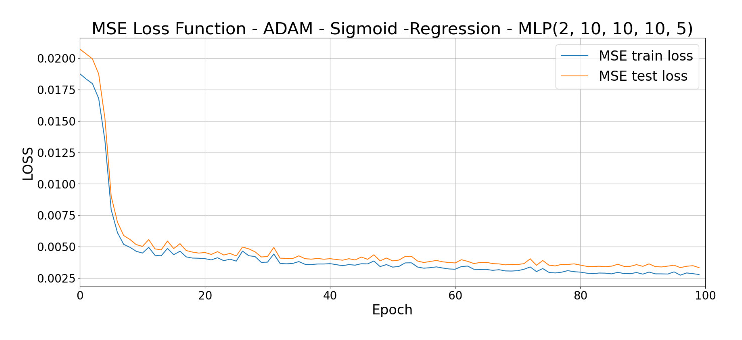
\includegraphics[width=1\linewidth]{MSE-Evolution.eps}
    \caption{MSE evolution of MLP-R}
    \label{mse}
\end{figure}



%%%%%%%%%%%%%%%%%%%%%%%%%%%%%%%%%%%%%%%%%%%%%%%%%%%%%%%%%%%%%%%%%%%%%%%%%%%%%%%%
\subsection{Inverse Mapping and Identification of Candidate MOFs}
%%%%%%%%%%%%%%%%%%%%%%%%%%%%%%%%%%%%%%%%%%%%%%%%%%%%%%%%%%%%%%%%%%%%%%%%%%%%%%%%

After determining that the MLP-R produces adequate results, it can be 
used as an inverse mapping tool. As mentioned before, the main goal of this 
method should be to calculate the structural parameters of a MOF (outputs) for 
given $\ugc$ and $\uvc$ (inputs). The response of the method might not be a 
specific MOF that will allow us to build a practical storage tank for a FCV. 
However, this method could report the ranges or intervals of values of the 
structural parameters of MOFs whose usable capacities are equal or larger than 
the DOE targets or close to them (See Fig.~\ref{ANN_MOFs_Solution}). In this 
sense, the MLP-R should be understood as a guiding tool to delimit 
promising regions or intervals of the structural parameters space, rather than 
as a generator of explicit MOFs.

\begin{figure}[ht]
    \centering
    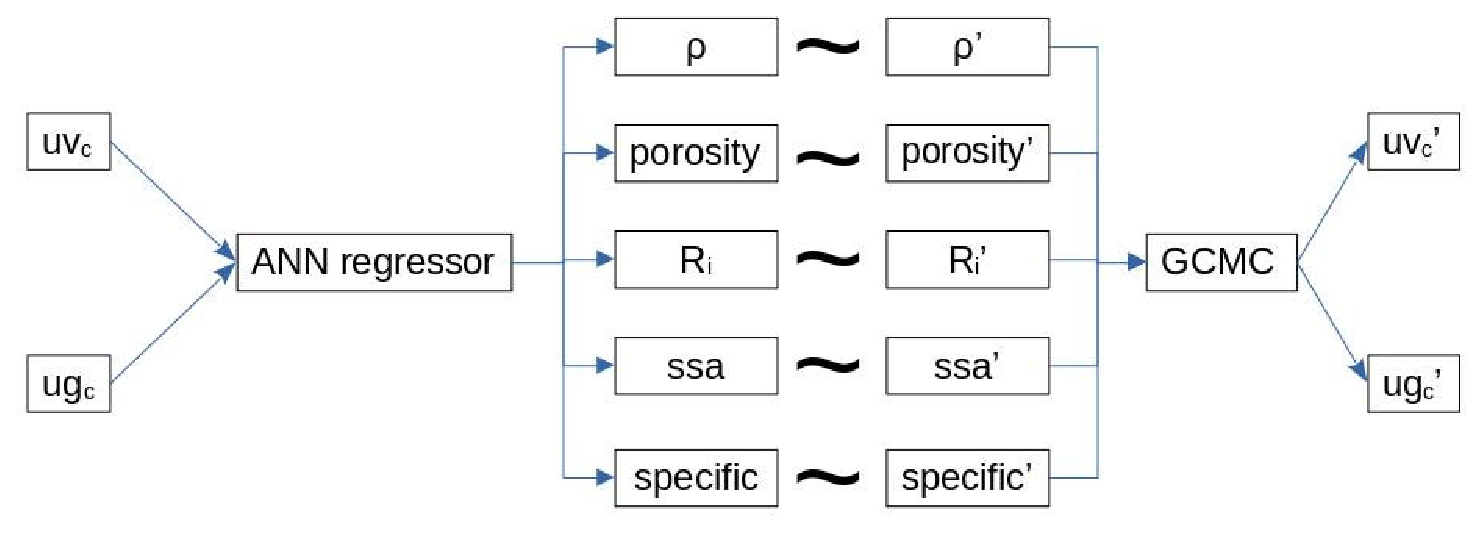
\includegraphics[width=1\linewidth]{Figura-Esquema-Recortado.eps}
    \caption{ANN output as starting point to search a MOFs solution}
    \label{ANN_MOFs_Solution}
\end{figure}

To illustrate the application of the inverse mapping strategy, two representative 
pairs of usable gravimetric and volumetric capacities were selected. The first 
pair was $\ugc$ and $\uvc$ of 2.75 wt. \% and 
0.04 kg/L, respectively. In this pair, the $\ugc$ was one half of the DOE 2025 
target and the $\uvc$ was the exact DOE 2025 volumetric target. The second 
representative pair was the exact DOE 2025 targets. These pairs were the 
inputs of the MLP-R and the structural parameters were the outputs. 
Table~\ref{outputs} summarize the MOFs structural parameters as output, according 
to the two representative pairs of given (or input) hydrogen $\ugc$ and $\uvc$, 
using the MLP-R and obtained using and omitting the Hold-Out methodology.

\begin{table}[H]
    \centering
    \begin{tabular}{ccccccc}
    \hline
\multicolumn{7}{c}{Hold-Out Outputs}\\
\hline
         $\ugc$   & $\uvc$   & density  & porosity & $R_i$ & SSA  & SPV\\
         2.75     & 0.04     & 0.597    & 0.413    & 5.69  & 3562 & 0.567\\
         5.50     & 0.04     & 0.386    & 0.673    & 8.37  & 5166 & 2.125\\
    \hline
\multicolumn{7}{c}{No Hold-Out Outputs}\\
\hline
         $\ugc$   & $\uvc$   & density  & porosity & $R_i$ & SSA  & SPV\\
         2.75     & 0.04     & 1.058    & 0.344    & 4.83  & 2772 & 0.282\\
         5.50     & 0.04     & 0.416    & 0.645    & 8.03  & 4810 & 1.717\\
    \hline
    \end{tabular}
    \caption{Hold-Out and No Hold-Out Outputs. 
    $\ugc$, $\uvc$, density, $R_i$, 
    SSA and SPV are in wt. \%, kg/L, kg/L, \AA{}, m$^2$/g and cm$^3$/g, 
    respectively. Porosity is dimensionless
    }
    \label{outputs}
\end{table}

According to the MLP-R \textcolor{blue}{method}, to reach the first pair of 
targets (2.75 wt. \%, 0.04 kg/L), the density should be about 0.6-1.1 kg/L and 
the porosity about 0.3-0.4 and the radius of the largest pore, the specific 
surface area and the specific pore volume of the MOF should be about 5 \AA{}, 
3000 m$^2$/g and 0.3-0.6 cm$^3$/g, respectively. As regards the second pair of 
targets (5.5 wt. \%, 0.04 kg/L), the density, porosity, largest pore radius, 
specific surface area and specific pore volume should be about 0.4 kg/L, 0.65, 
8 \AA{}, 5000 m$^2$/g and 2 cm$^3$/g, respectively. These values indicate that 
the materials, MOFs in this case, must be light and porous, a fact already well 
established in the scientific literature. The MLP regressor yields specific 
intervals of the structural parameters as a guide for the experimentalists to 
synthesize MOFs. 

The outputs of the MLP regressor are structural parameters, based on the two 
pairs of targets, but they are not specific MOFs. On the other hand, the MSE 
and R$^2$ values of the MLP regressor indicated the quality of the regressor to 
predict the structural parameters of MOFs. A procedure to ``predict'' specific 
MOFs and also to make additional tests of the quality of the MLP regressor 
consists on performing GCMC simulations of the storage capacities of MOFs whose 
structural parameters are similar to those predicted by the MLP regressor 
and comparing the predicted and the calculated storage capacities. Based 
on the predicted structural parameters in Table~\ref{outputs}, MOFs with 
similar characteristics were identified within the CCDC database. These 
candidate or selected MOFs were not among the \sout{1000} \textcolor{blue}{5000} 
MOFs used in the original dataset of 
the present study. GCMC simulations were then performed for these selected 
MOFs at 298.15 K and 25 MPa in order to evaluate their hydrogen storage 
capacities. The CCDC identifiers of these selected MOFs and their structural 
parameters and usable storage capacities are reported in Table~\ref{mofs}. 



\begin{table}[H]
\begin{center}
\caption{\noindent
\label{mofs} 
Structural parameters, usable capacities at 298.15 \textcolor{red}{K} and 25 MPa of the 
selected MOFs and driving range (in km) of an Adsorbed Hydrogen Gas, AHG, 
vehicle with the selected MOFs. Parameters include framework 
density, ($\rho$, kg/L), porosity, (Prs., dimensionless), largest pore radius, 
($R_i$, \AA{}), specific surface area (SSA, m$^2$/g), specific pore volume (SPV, 
cm$^3$/g), usable gravimetric capacity ($\ugc$, wt.\%), and usable volumetric 
capacity ($\uvc$, kg/L).}
\begin{tabular}{ccccccccc}
\hline
\diagbox{MOF}{Properties} & \textbf{Prs.} & \textbf{$\rho$} & \textbf{$R_i$} & \textbf{SSA} & \textbf{SPV} & \textbf{$\uvc$} & \textbf{$\ugc$} & \textbf{Driving Range}\\
\hline
ALEJAE            &  0.694 &  0.283  &  11.20  & 4795 & 2.544 & 0.0162 & 5.40 & 664 \\
BAZFUFf01         &  0.566 &  0.357  &  11.25  & 5192 & 1.678 & 0.0157 & 4.20 & 644 \\
BAZFUF            &  0.567 &  0.355  &  11.33  & 5141 & 1.744 & 0.0158 & 4.25 & 648 \\
BIBXOB            &  0.541 &  0.408  &  11.07  & 4641 & 1.518 & 0.0159 & 3.75 & 652 \\
BIHBAX            &  0.688 &  0.334  &   9.96  & 4396 & 2.034 & 0.0173 & 4.92 & 710 \\
BOGNES            &  0.429 &  0.415  &  10.31  & 5649 & 1.012 & 0.0136 & 3.18 & 558 \\
DAJWET            &  0.621 &  0.295  &  14.88  & 4985 & 2.509 & 0.0154 & 4.98 & 632 \\
DIMBOT            &  0.746 &  0.430  &  14.99  & 1903 & 1.722 & 0.0166 & 3.72 & 681 \\
ECOKAJ            &  0.682 &  0.333  &   8.97  & 3838 & 2.038 & 0.0153 & 4.39 & 628 \\
EHIJAH            &  0.574 &  0.385  &  10.38  & 4590 & 1.662 & 0.0152 & 3.80 & 623 \\
FE-PBPTA          &  0.669 &  0.411  &  10.09  & 4337 & 1.654 & 0.0179 & 4.17 & 734 \\
IRMOF-1\_MOF-5    &  0.380 &  0.598  &   7.53  & 3910 & 0.635 & 0.0144 & 2.35 & 591 \\
IPUPOA            &  0.551 &  0.403  &  10.58  & 4795 & 1.338 & 0.0154 & 3.67 & 632 \\
JLU-MONT1\_JEYTEP &  0.802 &  0.192  &  14.53  & 6035 & 4.479 & 0.0162 & 7.77 & 664 \\
JLU-SOF2\_KODPIF  &  0.749 &  0.232  &  14.12  & 4513 & 3.280 & 0.0153 & 6.20 & 628 \\
JLU-SOF3\_KODPIF01&  0.747 &  0.151  &  11.54  & 7244 & 5.567 & 0.0164 & 9.83 & 673 \\
LEJCIO            &  0.612 &  0.326  &  10.35  & 5126 & 1.961 & 0.0156 & 4.56 & 640 \\
OMUSAS            &  0.601 &  0.361  &   7.83  & 3823 & 1.663 & 0.0140 & 3.75 & 574 \\
OPAWOT            &  0.566 &  0.368  &   7.03  & 4834 & 1.358 & 0.0153 & 4.00 & 628 \\
UQOLUJ01          &  0.613 &  0.357  &  10.14  & 4834 & 1.622 & 0.0156 & 4.19 & 640 \\
VETMIS            &  0.609 &  0.321  &   5.11  & 5463 & 2.301 & 0.0155 & 4.59 & 636 \\
XAHPUT            &  0.755 &  0.186  &  11.83  & 5870 & 4.088 & 0.0162 & 8.01 & 664 \\
XAHQAA            &  0.779 &  0.176  &  12.31  & 5833 & 4.320 & 0.0164 & 8.52 & 673 \\
XANLIJ            &  0.692 &  0.231  &  13.73  & 5707 & 3.030 & 0.0154 & 6.25 & 632 \\
\hline
\end{tabular}
\end{center}
\end{table}


\textcolor{red}{
Several of the frameworks listed in Table~\ref{mofs} have previously been 
investigated for applications beyond hydrogen storage. For example, DUT-13 
(EHIJAH) (Zn$_4$O(BenzTB)$_{3/2}$) is characterized by a high pore volume and 
adsorption-induced structural flexibility, exhibiting framework opening upon 
adsorption of N$_2$ (-196~$^\circ$C), CO$_2$ (-78~$^\circ$C), and 
$n$-C$_4$H$_{10}$ (20~$^\circ$C) \cite{gsbk+11}.}
\textcolor{red}{
In the context of gas separation, PCP-32 (IPUPOA) combines high surface areas 
with a significant density of open metal sites, enabling efficient separation 
of C$_2$H$_2$/CO$_2$ mixtures at 298~K \cite{dhzn+17}. Likewise, JLU-SOF2 and 
JLU-SOF3 show high CO$_2$ uptake under ambient conditions together with 
preferential adsorption over N$_2$ and CH$_4$, demonstrating their potential 
for selective gas separation processes \cite{zkel+19}.}
\textcolor{red}{
Beyond gas-phase applications, some of these materials have also been explored 
in liquid-phase adsorption. JLU-MONT1 (JEYTEP) has been reported to exhibit 
remarkable adsorption capacity toward carcinogenic dyes such as BR9 and BV14 
\cite{zyml+18}, while other stable porous frameworks (VETMIS) have shown 
promising performance in adsorptive desulfurization with good recyclability 
\cite{llsx12}.
}



%%%%%%%%%%%%%%%%%%%%%%%%%%%%%%%%%%%%%%%%%%%%%%%%%%%%%%%%%%%%%%%%%%%%%%%%%%%%%%%%
\subsection{\textcolor{red}{Comparison with Reported Experimental Hydrogen 
Storage Data}}
%%%%%%%%%%%%%%%%%%%%%%%%%%%%%%%%%%%%%%%%%%%%%%%%%%%%%%%%%%%%%%%%%%%%%%%%%%%%%%%%

\textcolor{red}{To evaluate the predictive reliability of the computational 
framework, \textcolor{blue}{two groups of} comparisons with independent 
experimental measurements were performed. Well-established MOFs frequently used 
as reference materials in hydrogen adsorption studies were selected from the 
\sout{literature.} \textcolor{blue}{literature, to perform the first group of 
comparisons.} For each compound, adsorption \textcolor{blue}{GCMC} simulations 
were carried out under the same pressure and temperature conditions reported 
experimentally. This one-to-one correspondence in thermodynamic variables 
allows a direct assessment of the accuracy and transferability of the 
simulation protocol.}

\textcolor{red}{The experimental benchmarks and the corresponding simulation 
outcomes are collected in Table~\ref{comparisonH2}. The table lists hydrogen 
uptake values reported in the literature together with the results obtained in 
the present work using the mcmgs implementation of the GCMC method 
\cite{mcmgs}. All simulated values were generated under the same operating 
conditions as in the experiments to enable a direct comparison.
}



\begin{table}[H]
\begin{center}
\caption{\noindent
\label{comparisonH2}
Literature-reported hydrogen adsorption data for representative MOFs compared 
with \sout{Grand Canonical Monte Carlo} \textcolor{blue}{GCMC} results obtained 
in this work using the \texttt{mcmgs} code \cite{mcmgs}. Simulations were 
conducted at the same pressures and temperatures as the corresponding 
experiments to enable direct benchmarking. Pressure ($P$) is expressed in MPa 
and temperature ($T$) in K. Gravimetric uptake ($g_c$) is given in wt. \% and 
volumetric uptake ($v_c$) in kg/L. The column ``Type'' specifies whether total 
or excess adsorption is reported.
}
\bigskip
\begin{tabular}{cccccccc}
\hline
MOF          &  P   &  T  & Technique & $g_c$ & $v_c$  & Type   & Source \\
\hline
			IRMOF-1      &  3.5 &  77 & exps.     &  5.75 &      - & Excess & Zhou et al. \cite{zwhy07} \\
			IRMOF-1      &  3.5 &  77 & mcmgs     &  5.34 &      - & Excess & Granja-DelRío and Cabria \cite{gc24b} \\
			IRMOF-1      &  4.8 &  77 & exps.     &  5.2  &      - & Total  & Collins and Zhou \cite{cz07} \\
			IRMOF-1      &  4.8 &  77 & mcmgs     &  6.7  &      - & Total  & Granja-DelRío and Cabria \cite{gc24b} \\
			IRMOF-1      &  6   &  77 & exps.     &  5.6  &	     - & Excess & Zhou et al. \cite{zwhy07} \\
			IRMOF-1      &  6   &  77 & mcmgs     &  5.7  &	     - & Excess & Granja-DelRío and Cabria \cite{gc24b} \\
			IRMOF-1      &  6   & 298 & exps.     &  0.45 &	     - & Total  & Collins and Zhou \cite{cz07} \\
			IRMOF-1      &  6   & 298 & mcmgs     &  0.72 &	     - & Total  & Granja-DelRío and Cabria \cite{gc24b} \\
			IRMOF-1      &  6   & 298 & exps.     &  0.45 &      - & Excess & Collins and Zhou\cite{cz07} \\
			IRMOF-1      &  6   & 298 & mcmgs     &  0.38 &      - & Excess & Granja-DelRío and Cabria \cite{gc24c} \\
			IRMOF-1      & 10   & 298 & exps.     &  0.45 &	     - & Excess & Yang et al. \cite{yki+12} \\
			IRMOF-1      & 10   & 298 & mcmgs     &  0.58 &      - & Excess & Granja-DelRío and Cabria \cite{gc24c}\\
			IRMOF-1      & 10   & 298 & exps.     &  0.42 &	     - & Excess & Langmi et al. \cite{lrnmb14} \\
			IRMOF-1      & 10   & 298 & mcmgs     &  0.58 &      - & Excess & Granja-DelRío and Cabria \cite{gc24c}\\
			IRMOF-1      &  6   & 300 & exps.     &  0.3  &	     - & Excess & Zhou et al. \cite{zwhy07} \\
			IRMOF-1      &  6   & 300 & mcmgs     &  0.37 &	     - & Excess & Granja-DelRío and Cabria \cite{gc24a}\\
			\hline
			IRMOF-20     &  2   &  77 & exps.     &  6.38 &  0.035 & Total  & Ahmed et al. \cite{asp+19} \\
			IRMOF-20     &  2   &  77 & mcmgs     &  6.82 &  0.048 & Total  & Present work\\
			IRMOF-20     &  6   &  77 & exps.     &  8.43 &  0.047 & Total  & Ahmed et al. \cite{asp+19} \\
			IRMOF-20     &  6   &  77 & mcmgs     &  8.12 &  0.058 & Total  & Present work\\
			IRMOF-20     & 10   &  77 & exps.     &  9.26 &  0.052 & Total  & Ahmed et al. \cite{asp+19} \\
			IRMOF-20     & 10   &  77 & mcmgs     &  8.65 &  0.062 & Total  & Present work\\	
			\hline
			ZIF-8        &  3   &  77 & exps.     &  3.3  &	     - & Excess & Zhou et al. \cite{zwhy07} \\
			ZIF-8        &  3   &  77 & mcmgs     &  2.74 &      - & Excess & Granja-DelRío and Cabria \cite{gc24b} \\
			ZIF-8        &  5   &  77 & exps.     &  3.2  &	     - & Excess & Zhou et al. \cite{zwhy07} \\
			ZIF-8        &  5   &  77 & mcmgs     &  2.86 &	     - & Excess & Granja-DelRío and Cabria \cite{gc24b} \\
			ZIF-8        &  5   & 300 & exps.     &  0.1  &	     - & Excess & Zhou et al. \cite{zwhy07} \\
			ZIF-8        &  5   & 300 & mcmgs     &  0.18 &	     - & Excess & Granja-DelRío and Cabria \cite{gc24b} \\
			\hline
		\end{tabular}
	\end{center}
\end{table}

\textcolor{red}{
Overall, the simulated \sout{adsorption} \textcolor{blue}{storage} capacities 
reproduce the main experimental trends with reasonable fidelity 
(Table~\ref{comparisonH2}). Differences between computed and measured values 
remain within the expected range for classical force‑field‑based GCMC. In 
several cases, the simulated \sout{uptakes} \textcolor{blue}{storage 
capacities} are moderately higher than the experimental ones (typically 20-30 
\%), which is commonly attributed to uncertainties in force‑field 
parametrization, framework rigidity assumptions, and experimental conditions.
}

\textcolor{blue}{In the second group of comparisons, the experimental and GCMC 
capacities of MOFs selected from 
Table~\ref{mofs} are compared}. \textcolor{red}{In order to 
identify suitable experimental benchmarks, the MOFs listed in 
\sout{Table~\ref{mofs}} \textcolor{blue}{that Table} were systematically 
examined in the literature. Most of these materials have been synthesized and 
characterized for applications such as gas separation or liquid-phase 
adsorption, but experimental hydrogen adsorption data under controlled 
thermodynamic conditions remain scarce. Among all the frameworks in 
Table~\ref{mofs}, \sout{only} \textcolor{blue}{IRMOF-1 and} DUT-13 (EHIJAH) 
\sout{was} \textcolor{blue}{were} found to have reported hydrogen 
adsorption measurements suitable for \sout{direct} comparison with the present 
simulations. 
\textcolor{blue}{These two datasets were, therefore, selected  
as representative cases for benchmarking the 
simulation workflow within the set of candidate MOFs identified by the ANN.}
\sout{These measurements correspond to excess gravimetric hydrogen 
adsorption at 77~K and pressures up to about 10~MPa \cite{gsbk+11}. The DUT-13 
dataset was therefore selected as a representative case for benchmarking the 
simulation workflow within the set of candidate MOFs identified by the ANN.
}}

\textcolor{blue}{The comparison is not direct, due to the scarce number of 
experiments at 25 MPa and room temperature. The measurements of DUT-13 
correspond to excess gravimetric hydrogen adsorption at 77~K and pressures up 
to about 10~MPa \cite{gsbk+11} and those of IRMOF-1 correspond to total 
capacities at 6 MPa and 298 K \cite{cz07}.}
\textcolor{red}{In the context of porous materials, excess adsorption is 
defined as the quantity of gas retained in the pores beyond the amount that 
would occupy the same \sout{free} volume at the bulk gas density. It therefore 
isolates the contribution arising from solid–fluid interactions and excludes 
the purely compressible gas phase. Because this definition captures the 
intrinsic adsorption strength of a framework, excess uptake is widely adopted 
as a reference metric for inter-material comparison.}

\sout{
\textcolor{red}{A comparison with the experimental dataset of Sengupta et 
al.~\cite{smbd+23} was conducted under matching conditions, with GCMC 
simulations at 296~K over the same pressure range; the 
resulting total volumetric hydrogen capacities from both 
sources are displayed in panel~a) of Fig.~\ref{h277K}.}
}



\begin{figure}[htpb]
\vspace{0.0cm}
\begin{center}
\leavevmode
\includegraphics[width=\len cm]{DUT-13-gc.eps}
\end{center}
\vspace{-0.5cm}
\caption{
\textcolor{red}{Excess hydrogen gravimetric capacity isotherms at 77~K 
for DUT-13 (EHIJAH). The experimental points follow the pressure values 
reported by Grünker et al.~\cite{gsbk+11}. The curves obtained with the mcmgs 
code are included for comparison (red)} 
}
\label{h277K}
\end{figure}



\sout{
\textcolor{blue}{The experimental total volumetric hydrogen capacities reported 
by Sengupta et al.~\cite{smbd+23} and those obtained from the GCMC simulations 
exhibit very similar trends for the MOF NU-2100 at 296~K (See 
Figure~\ref{h277K}a). The experimental and GCMC capacities increase smoothly 
with pressure, and both isotherms or curves have the same general shape.} 
\textcolor{red}{\sout{Figure~\ref{h277K}a shows that the total volumetric 
hydrogen capacities reported by Sengupta et al.~\cite{smbd+23} and those 
obtained from the mcmgs simulations exhibit very similar trends for the MOF 
NU-2100 at 296~K. In both cases, the capacity increases smoothly with pressure, 
and the experimental curves retain the same general shape as the simulated 
ones.} Quantitatively, the volumetric capacity values coincide within 
uncertainty up to about 4~MPa. Above this pressure, a systematic offset 
appears: the simulated capacities exceed the experimental data by approximately 
0.001~kg/L, which corresponds to roughly 14 \%. Thus, while 
\textcolor{blue}{the} agreement is good in the low-pressure regime and both 
curves remain close, the simulated values grow slightly faster at higher 
pressures, leading to a moderate, nearly constant deviation in the 
high-pressure region. Overall, the comparison confirms consistent low‑pressure 
behavior and a small, pressure-dependent spread at higher pressures for total 
volumetric capacity.}
}

\textcolor{red}{
Figure~\ref{h277K} shows the excess gravimetric hydrogen capacities at 77~K for 
DUT-13 (EHIJAH) reported by Grünker et al.~\cite{gsbk+11} together with the 
results obtained from the mcmgs simulations. In both cases, the gravimetric 
capacity increases with pressure and reaches a maximum at approximately 
5-6~MPa. The experimental data show a maximum hydrogen uptake of 
5.23~wt.\% at 5.6~MPa, whereas the simulations predict a maximum value close 
to 7~wt.\% near 6~MPa.
}

\textcolor{red}{
For DUT-13, the simulated capacities of DUT-13 are systematically higher than the 
experimental values. The agreement is reasonably good. 
At 10~MPa, the simulated capacity exceeds the experimental value by about only
28~\%. Despite this deviation, both curves exhibit a similar shape and a 
consistent pressure dependence. The comparison therefore supports the 
ability of the mcmgs workflow to reproduce the main adsorption trends for 
DUT-13 at cryogenic temperature.}
\textcolor{blue}{
As regards IRMOF-1, the GCMC total gravimetric capacity is also higher than the 
experimental capacity at 6 MPa and 298 K. The experimental total gravimetric capacities 
differ by about 60 \%, as can be noticed in Table~\ref{comparisonH2}.}



%%%%%%%%%%%%%%%%%%%%%%%%%%%%%%%%%%%%%%%%%%%%%%%%%%%%%%%%%%%%%%%%%%%%%%%%%%%%%%%%
\subsection{\textcolor{red}{Driving range of a vehicle}}
%%%%%%%%%%%%%%%%%%%%%%%%%%%%%%%%%%%%%%%%%%%%%%%%%%%%%%%%%%%%%%%%%%%%%%%%%%%%%%%%

Besides of the calculation of the storage capacities of the selected MOFs, 
the driving range of an AHG vehicle was also calculated (See Table~\ref{mofs}). 
If a selected MOF 
is incorporated into an Adsorbed Hydrogen Gas, AHG, storage system within 
the same vehicle and with a total volume of 2.5 x 142 = 355 litres, the 
driving range in km of the AHG vehicle will be $\uvc$ x 355 litres x 647 
km / 5.6 kg, where $\uvc$ is in kg/L units. That driving range is shown in 
the last column in Table~\ref{mofs} for the selected MOFs. To illustrate 
the potential system-level implications of the storage capacities of the 
selected MOFs, a simplified comparison with a commercial hydrogen fuel cell 
vehicle was carried out. The 2024 Toyota Mirai was selected as a reference 
system due to the availability of public technical data. The hydrogen storage 
system of the 2024 Toyota Mirai, a hydrogen fuel cell vehicle, consists of 
tanks with a total volume of 142 litres, stores 5.6 kg of hydrogen at 70 MPa 
and the vehicle has a driving range of 402 miles (647 km) \cite{toyota24}. 
Hence, in the calculation of the driving range of an AHG vehicle with the 
selected MOFs, the ratio 647 km / 5.6 kg was used in order to have a vehicle 
with the same engine efficiency as the Toyota Mirai 2024 and then, a proper 
comparison could be carried out. 
 
It can be noticed in Table~\ref{mofs} that most of selected MOFs have 
a usable gravimetric capacity that reaches the DOE gravimetric target 
for 2025 and a driving range, with a 355 litres storage AHG tank system, 
that reaches or is close to the driving range of an existing FCV, the 2024 
Toyota Mirai. However, their usable volumetric capacities remain below the 
DOE requirement. For this reason, the comparison with the 2024 Toyota Mirai 
is presented only as an illustrative system-level analysis. 
 
Using an AHG storage system operating at 25 MPa, an internal tank volume of 355 
litres (i.e., approximately 2.5 times the volume of the compressed-gas system 
at 70 MPa) would be required to achieve a driving range comparable to that 
of the Mirai.  These results highlight that, within the explored structural 
space, the ML model does not identify MOFs that simultaneously satisfy both the 
gravimetric and volumetric DOE targets at moderate pressure. Nevertheless, 
operating at lower pressure (25 MPa instead of 70 MPa) offers practical 
advantages, including reduced system cost, improved safety margins, enhanced 
durability, and lower maintenance requirements. The disadvantage is a large 
volume for the storage system. This could be a viable, although not perfect 
technological solution. Future extensions of this approach may explore 
broader structural spaces or alternative operating conditions to further 
improve volumetric performance. 



%%%%%%%%%%%%%%%%%%%%%%%%%%%%%%%%%%%%%%%%%%%%%%%%%%%%%%%%%%%%%%%%%%%%%%%%%%%%%%%%
\section{Conclusions}
%%%%%%%%%%%%%%%%%%%%%%%%%%%%%%%%%%%%%%%%%%%%%%%%%%%%%%%%%%%%%%%%%%%%%%%%%%%%%%%%

Leveraging Artificial Intelligence, a MLP regressor, a type of ANN method, was 
designed to act as a nonlinear function estimator for hydrogen storage 
capacities characterized by complex structure-property relationships. From a 
computational standpoint, it can be categorized as an intelligent system within 
the field of Soft Computing, given its relatively low resource consumption. 
The MLP regressor was trained to identify regions or intervals of the 
structural parameters of MOFs whose hydrogen usable storage capacities are 
equal or larger than the DOE 2025 targets. The database used to train the 
MLP regressor contained the usable gravimetric and volumetric capacities 
at 25 MPa and 298.15 K of the MOFs and \sout{five} \textcolor{blue}{eight} 
structural parameters: density, porosity, largest pore radius, specific surface 
\sout{area and specific pore volume.} \textcolor{blue}{area, specific pore 
volume, the degree of unsaturation, the metal weight percentage and the metal 
atom percentage.}
 
The main novelty of the work consisted on applying the MLP regressor to predict 
or identify regions of structural parameters of MOFs whose usable storage 
capacities at 25 MPa and 298.15 K match specific values, the DOE 2025 targets, 
instead of predicting usable storage capacities from given MOF structures. 
The specific predictions of the model are that the density, porosity, largest 
pore radius, specific surface \sout{area and specific pore volume} 
\textcolor{blue}{area, specific pore volume, the degree of unsaturation, the
metal weight percentage and the metal atom percentage} should \sout{be about 
0.4 kg/L, 0.65, 8 \AA{}, 5000 m$^2$/g and 2 cm$^3$/g, respectively,} 
\textcolor{blue}{be about x kg/L, y, z \AA{}, a m$^2$/g, c cm$^3$/g, du, mw \% 
and ma \% respectively,} in order to reach the DOE 2025 targets. These 
parameters strongly influence both the usable gravimetric and volumetric 
hydrogen storage capacities. These regions of structural parameters can help 
experimental researchers to focus their synthesis efforts on MOFs showing 
combinations of these structural properties that are more likely to achieve the 
DOE requirements. 
 
GCMC simulations were performed on MOFs close to these predicted regions, not 
included in the original database used for the training of the MLP regressor. 
The usable gravimetric capacity of most of these selected MOFs equals or 
exceeds the DOE 2025 target. In contrast, the usable volumetric capacity 
remains approximately half of the required value. An AHG vehicle using these 
MOFs could achieve a driving range comparable to that of the 2024 Toyota 
Mirai using a storage volume about 2.5 times larger. This finding clarifies 
that the proposed approach does not meet the DOE 2025 volumetric target at 
moderate pressure, 25 MPa compared to 70 MPa, but it delineates realistic 
trade-offs between storage volume, operating pressure, and system-level 
performance. Lower-pressure operation provides relevant system-level 
advantages, including reduced cost, improved durability, enhanced safety, and 
lower maintenance requirements, which are important considerations for the 
practical deployment of hydrogen storage technologies. 



%%%%%%%%%%%%%%%%%%%%%%%%%%%%%%%%%%%%%%%%%%%%%%%%%%%%%%%%%%%%%%%%%%%%%%%%%%%%%%%%
\section{Acknowledgments}
%%%%%%%%%%%%%%%%%%%%%%%%%%%%%%%%%%%%%%%%%%%%%%%%%%%%%%%%%%%%%%%%%%%%%%%%%%%%%%%%
This work was supported by financial aid from the Spanish Ministry of Science 
and Innovation (Project PGC2018-093745-B-I00), the Regional Government of 
Castilla y León (Project VA124G18), and the University of Valladolid. The use 
of the computing resources offered by the Data Processing Center at the Science 
Park of the University of Valladolid is also recognized.



%%%%%%%%%%%%%%%%%%%%%%%%%%%%%%%%%%%%%%%%%%%%%%%%%%%%%%%%%%%%%%%%%%%%%%%%%%%%%
% Bibliography
%%%%%%%%%%%%%%%%%%%%%%%%%%%%%%%%%%%%%%%%%%%%%%%%%%%%%%%%%%%%%%%%%%%%%%%%%%%%%

%\bibliographystyle{elsarticle-num} %% `Elsevier LaTeX' style
%\bibliography{../bibdatabase-suggested-referees/physicsandchemistry.bib}

\begin{thebibliography}{100}
\expandafter\ifx\csname url\endcsname\relax
  \def\url#1{\texttt{#1}}\fi
\expandafter\ifx\csname urlprefix\endcsname\relax\def\urlprefix{URL }\fi
\expandafter\ifx\csname href\endcsname\relax
  \def\href#1#2{#2} \def\path#1{#1}\fi

\bibitem{zjb+24}
L.~Zhang, C.~Jia, F.~Bai, W.~Wang, S.~An, K.~Zhao, Z.~Li, J.~Li, H.~Sun, A
  comprehensive review of the promising clean energy carrier: Hydrogen
  production, transportation, storage, and utilization {(HPTSU)} technologies,
  Fuel 355 (2024) 129455.
\newblock \href {https://doi.org/10.1016/j.fuel.2023.129455}
  {\path{doi:10.1016/j.fuel.2023.129455}}.

\bibitem{cde+22}
S.~Chakraborty, S.~K. Dash, R.~M. Elavarasan, A.~Kaur, D.~Elangovan, S.~T.
  Meraj, P.~Kasinathan, Z.~Said, Hydrogen energy as future of sustainable
  mobility, Front. Energy Res. 10 (2022) 893475.
\newblock \href {https://doi.org/10.3389/fenrg.2022.893475}
  {\path{doi:10.3389/fenrg.2022.893475}}.

\bibitem{jena11}
P.~Jena, Materials for hydrogen storage: Past, present, and future, J. Phys.
  Chem. Lett. 2~(3) (2011) 206--211.
\newblock \href {https://doi.org/10.1021/jz1015372}
  {\path{doi:10.1021/jz1015372}}.

\bibitem{tm24}
{European Environment Agency}, Transport and mobility,
  https://www.eea.europa.eu/en/topics/in-depth/transport-and-mobility,
  {Accessed January 2, 2026} (2024).

\bibitem{netzeroiea}
{IEA}, {Net Zero by 2050. A Roadmap for the Global Energy Sector},
  https://www.iea.org/reports/net-zero-by-2050, {Accessed February 7, 2026}
  (2021).

\bibitem{netzerousa}
{United States Department of State and the United States Executive Office of
  the President}, The long-term strategy of the {U}nited {S}tates, pathways to
  net-zero greenhouse gas emissions by 2050,
  https://unfccc.int/sites/default/files/resource/US-LongTermStrategy-2021.pdf,
  {Accessed February 7, 2026} (2021).

\bibitem{smcf20}
G.~Sdanghi, G.~Maranzana, A.~Celzard, V.~Fierro, Towards non-mechanical hybrid
  hydrogen compression for decentralized hydrogen facilities, Energies 13~(12)
  (2020) 3145.
\newblock \href {https://doi.org/10.3390/en13123145}
  {\path{doi:10.3390/en13123145}}.

\bibitem{doe25}
{Office of Energy Efficiency \& Renewable Energy, Fuel Cell Technologies
  Office}, {DOE} technical targets for onboard hydrogen storage for light-duty
  vehicles,
  https://www.energy.gov/eere/fuelcells/doe-technical-targets-onboard-hydrogen-storage-light-duty-vehicles,
  {Accessed January 2, 2026} (2018).

\bibitem{cstc22}
T.~Capurso, M.~Stefanizzi, M.~Torres, S.~M. Camporeale, Review perspective of
  the role of hydrogen in the 21st century energy transition, Energy Convers.
  Manag. 251 (2022) 114898.

\bibitem{apap19}
J.~O. Abe, A.~P.~I. Popoola, E.~Ajenifuja, O.~M. Popoola, Hydrogen energy,
  economy and storage: Review and recommendation, Int. J. Hydrogen Energy 44
  (2019) 15072--15086.
\newblock \href {https://doi.org/10.1016/j.ijhydene.2019.04.068}
  {\path{doi:10.1016/j.ijhydene.2019.04.068}}.

\bibitem{bw15}
M.~Ball, M.~Weeda, The hydrogen economy-vision or reality?, Int. J. Hydrogen
  Energy 40 (2015) 7903--7919.

\bibitem{bhlk+26}
O.~Bourzgui, A.~{El harrak}, E.~H. Lahrar, O.~{El Kssiri}, I.~Nadi, A.~Faik,
  Toward scalable hydrogen storage in mobility systems: An integrated review of
  metal hydrides, multiscale modeling, and sustainability assessment, J. Power
  Sources 670 (2026) 239448.
\newblock \href {https://doi.org/10.1016/j.jpowsour.2026.239448}
  {\path{doi:10.1016/j.jpowsour.2026.239448}}.

\bibitem{laaz+25}
J.~A. Lenis, J.~{Arias Velandia}, R.~{Aguirre Ocampo}, A.~A. {Zuleta Gil},
  S.~Bello, E.~Correa, C.~Arrieta, F.~J. Bolívar, F.~{Echeverría
  Echeverría}, Challenges and potential future trends on high entropy alloy
  for solid hydrogen storage: Systematic review, J. Power Sources 656 (2025)
  238011.
\newblock \href {https://doi.org/10.1016/j.jpowsour.2025.238011}
  {\path{doi:10.1016/j.jpowsour.2025.238011}}.

\bibitem{atd20}
G.~Assoualaye, A.~Tom, N.~Djongyang, Monte {C}arlo study of hydrogen adsorption
  by {MOF-5} doped with cobalt at ambient temperature and pressure, SN Appl.
  Sci. 2 (2020) 1815.
\newblock \href {https://doi.org/10.1007/s42452-020-03627-9}
  {\path{doi:10.1007/s42452-020-03627-9}}.

\bibitem{hv14}
H.~T. Hwang, A.~Varma, Hydrogen storage for fuel cell vehicles, Curr. Opin.
  Chem. Eng. 5 (2014) 42--48.
\newblock \href {https://doi.org/10.1016/j.coche.2014.04.004}
  {\path{doi:10.1016/j.coche.2014.04.004}}.

\bibitem{cwlcz23}
C.~Chu, K.~Wu, B.~Luo, Q.~Cao, H.~Zhang, Hydrogen storage by liquid organic
  hydrogen carriers: Catalyst, renewable carrier, and technology – a review,
  Carbon Resour. Convers. 6~(4) (2023) 334--351.
\newblock \href {https://doi.org/10.1016/j.crcon.2023.03.007}
  {\path{doi:10.1016/j.crcon.2023.03.007}}.

\bibitem{rhs+22}
M.~G. Rasul, M.~A. Hazrat, M.~A. Sattar, M.~I. Jahirul, M.~J. Shearer, The
  future of hydrogen: Challenges on production, storage and applications,
  Energy Convers. Manag. 272 (2022) 116326.
\newblock \href {https://doi.org/10.1016/j.enconman.2022.116326}
  {\path{doi:10.1016/j.enconman.2022.116326}}.

\bibitem{breeze18}
P.~Breeze, Hydrogen energy storage, Elsevier, London, 2018, Ch.~8, pp. 69--77.

\bibitem{dy11}
F.~Ding, B.~I. Yakobson, Challenges in hydrogen adsorptions: from physisorption
  to chemisorption, Front. Phys. 6 (2011) 142--150.
\newblock \href {https://doi.org/10.1007/s11467-011-0171-6}
  {\path{doi:10.1007/s11467-011-0171-6}}.

\bibitem{bww+21}
D.~P. Broom, C.~J. Webb, K.~E. Webb, P.~A. Parilla, T.~Gennett, C.~M. Brown,
  R.~Zacharia, E.~Tylianakis, E.~Klontzas, G.~E. Froudakis, T.~A. Steriotis,
  P.~N. Trikalitis, D.~L. Anton, B.~Hardy, D.~Tamburello, C.~Corgnale, B.~A.
  van Hassel, D.~Cossement, R.~Chahine, M.~Hirscher, Outlook and challenges for
  hydrogen storage in nanoporous materials, Appl. Physics A 122 (2021) 151.
\newblock \href {https://doi.org/10.1007/s00339-016-9651-4}
  {\path{doi:10.1007/s00339-016-9651-4}}.

\bibitem{h2tanks}
{Office of Energy Efficiency \& Renewable Energy, Hydrogen and Fuel Cell
  Technologies Office}, {High-Pressure Hydrogen Tank Testing},
  https://www.energy.gov/eere/fuelcells/high-pressure-hydrogen-tank-testing,
  {Accessed January 2, 2026} (2022).

\bibitem{llk+22}
S.-Y. Lee, J.-H. Lee, Y.-H. Kim, J.-W. Kim, K.-J. Lee, S.-J. Park, Recent
  progress using solid-state materials for hydrogen storage: A short review,
  Processes 10 (2022) 304.
\newblock \href {https://doi.org/10.3390/pr10020304}
  {\path{doi:10.3390/pr10020304}}.

\bibitem{zuttel03}
A.~Z{\"u}ttel, Materials for hydrogen storage, Materials Today 6~(9) (2003)
  24--33.
\newblock \href {https://doi.org/10.1016/S1369-7021(03)00922-2}
  {\path{doi:10.1016/S1369-7021(03)00922-2}}.

\bibitem{ahg+18}
M.~D. Allendorf, Z.~Hulvey, T.~Gennett, A.~Ahmed, T.~Autrey, J.~Camp, E.~S.
  Cho, H.~Furukawa, M.~Haranczyk, M.~Head-Gordon, S.~Jeong, A.~Karkamkar, D.-J.
  Liu, J.~R. Long, K.~R. Meihaus, I.~H. Nayyar, R.~Nazarov, D.~J. Siegel,
  V.~Stavila, J.~J. Urban, S.~P. Veccham, B.~C. Wood, An assessment of
  strategies for the development of solid-state adsorbents for vehicular
  hydrogen storage, Energy Environ. Sci. 11 (2018) 2784--2812.
\newblock \href {https://doi.org/10.1039/C8EE01085D}
  {\path{doi:10.1039/C8EE01085D}}.

\bibitem{usdrivetarget2017}
P.~author, Target explanation document: Onboard hydrogen storage for light-duty
  fuel cell vehicles, Tech. rep., U.S. DRIVE Partnership (2017).

\bibitem{usdrivetarget17}
P.~author, Target explanation document: Onboard hydrogen storage for light-duty
  fuel cell vehicles, Tech. rep., U.S. DRIVE Partnership (2017).

\bibitem{doetables17}
P.~author, Technical system targets: Onboard hydrogen storage for light-duty
  fuel cell vehicles, Tech. rep., U.S. Department of Energy (2017).

\bibitem{ahluwalia24}
R.~K. Ahluwalia, D.~D. Papadias, J.-K. Peng, H.~S. Roh, System level analysis
  of hydrogen storage options (st001), 2024 doe hydrogen program annual merit
  review,
  {https://www.hydrogen.energy.gov/docs/hydrogenprogramlibraries/pdfs/review24/st001\_ahluwalia\_2024\_o.pdf}
  (2024).

\bibitem{hsecoe19}
M.~Thornton, L.~Simpson, System design, analysis, and modeling activities
  supporting the doe hydrogen storage engineering center of excellence
  (hsecoe): Final project report, Tech. Rep. NREL/TP-5400-73571, National
  Renewable Energy Laboratory (NREL) (2019).

\bibitem{ahp12}
R.~K. Ahluwalia, T.~Q. Hua, J.-K. Peng, On-board and off-board performance of
  hydrogen storage options for light-duty vehicles, International Journal of
  Hydrogen Energy 37 (2012) 2891--2910.
\newblock \href {https://doi.org/10.1016/j.ijhydene.2011.05.040}
  {\path{doi:10.1016/j.ijhydene.2011.05.040}}.

\bibitem{jbpr23}
R.~Jose, G.~Bangar, S.~Pal, G.~Rajaraman, Role of molecular modelling in the
  development of metal-organic framework for gas adsorption applications., J.
  Chem. Sci. 135 (2023) 19.
\newblock \href {https://doi.org/10.1007/s12039-022-02130-5}
  {\path{doi:10.1007/s12039-022-02130-5}}.

\bibitem{nasm22}
K.~Nath, A.~Ahmed, D.~J. Siegel, A.~J. Matzger, Computational identification
  and experimental demonstration of high-performance methane sorbents, Angew.
  Chem. Int. Ed. 61~(25) (2022) e202203575.
\newblock \href {https://doi.org/10.1002/anie.202203575}
  {\path{doi:10.1002/anie.202203575}}.

\bibitem{zwy+22}
D.~Zhao, X.~Wang, L.~Yue, Y.~He, B.~Chen, Porous metal–organic frameworks for
  hydrogen storage, Chem. Commun. 58 (2022) 11059--11078.
\newblock \href {https://doi.org/10.1039/D2CC04036K}
  {\path{doi:10.1039/D2CC04036K}}.

\bibitem{fvy+22}
K.~A. Forrest, G.~Verma, Y.~Ye, J.~Ren, S.~Ma, T.~Pham, B.~Space, Methane
  storage in flexible and dynamical metal–organic frameworks, Chem. Phys.
  Rev. 3~(2) (2022) 021308.
\newblock \href {https://doi.org/10.1063/5.0072805}
  {\path{doi:10.1063/5.0072805}}.

\bibitem{Li22}
A.~Li, Metal-organic frameworks-based hydrogen storage strategies and
  applications, J. Phys.: Conf. Ser. 2403~(1) (2022) 012022.
\newblock \href {https://doi.org/10.1088/1742-6596/2403/1/012022}
  {\path{doi:10.1088/1742-6596/2403/1/012022}}.

\bibitem{sap+21}
K.~Suresh, D.~Aulakh, J.~Purewal, D.~J. Siegel, M.~Veenstra, A.~J. Matzger,
  Optimizing hydrogen storage in {MOFs} through engineering of crystal
  morphology and control of crystal size, J. Am. Chem. Soc. 143~(28) (2021)
  10727--10734.
\newblock \href {https://doi.org/10.1021/jacs.1c04926}
  {\path{doi:10.1021/jacs.1c04926}}.

\bibitem{jje+21}
D.~E. Jaramillo, H.~Z.~H. Jiang, H.~A. Evans, R.~Chakraborty, H.~Furukawa,
  C.~M. Brown, M.~Head-Gordon, J.~R. Long, Ambient-temperature hydrogen storage
  via {Vanadium({II})}-dihydrogen complexation in a metal-organic framework, J.
  Am. Chem. Soc. 143~(16) (2021) 6248--6256.
\newblock \href {https://doi.org/10.1021/jacs.1c01883}
  {\path{doi:10.1021/jacs.1c01883}}.

\bibitem{ykc+18}
L.~Yuan, L.~Kang, Y.~Chen, D.~Wang, J.~Gong, C.~Wang, M.~Zhang, X.~Wu, Hydrogen
  storage capacity on {Ti}-decorated porous graphene: First-principles
  investigation, Appl. Surf. Sci. 434 (2018) 843--849.
\newblock \href {https://doi.org/10.1016/j.apsusc.2017.10.231}
  {\path{doi:10.1016/j.apsusc.2017.10.231}}.

\bibitem{wcd+18}
L.~Wang, X.~Chen, H.~Du, Y.~Yuan, H.~Qu, M.~Zou, First-principles investigation
  on hydrogen storage performance of {Li}, {Na} and {K} decorated borophene,
  Appl. Surf. Sci. 427 (2018) 1030--1037.
\newblock \href {https://doi.org/10.1016/j.apsusc.2017.08.126}
  {\path{doi:10.1016/j.apsusc.2017.08.126}}.

\bibitem{yck+17}
L.~Yuan, Y.~Chen, L.~Kang, C.~Zhang, D.~Wang, C.~Wang, M.~Zhang, X.~Wu,
  First-principles investigation of hydrogen storage capacity of {Y}-decorated
  porous graphene, Appl. Surf. Sci. 399 (2017) 463--468.
\newblock \href {https://doi.org/10.1016/j.apsusc.2016.12.054}
  {\path{doi:10.1016/j.apsusc.2016.12.054}}.

\bibitem{bd15}
M.~Beckner, A.~Dailly, Adsorbed methane storage for vehicular applications,
  Appl. Energy 149 (2015) 69--74.
\newblock \href {https://doi.org/10.1016/j.apenergy.2015.03.123}
  {\path{doi:10.1016/j.apenergy.2015.03.123}}.

\bibitem{doerecord25}
P.~author, Onboard type {IV} compressed hydrogen storage system-cost and
  performance status (program record 24006), Tech. rep., DOE Hydrogen Program
  (2025).

\bibitem{dbc22}
L.~Donà, J.~G. Brandenburg, B.~Civalleri, Metal-organic frameworks properties
  from hybrid density functional approximations, J. Chem. Phys. 156~(9) (2022)
  094706.
\newblock \href {https://doi.org/10.1063/5.0080359}
  {\path{doi:10.1063/5.0080359}}.

\bibitem{fgf22}
G.~S. Fanourgakis, K.~Gkagkas, G.~Froudakis, Introducing artificial {MOFs} for
  improved machine learning predictions: Identification of top-performing
  materials for methane storage, J. Chem. Phys. 156~(5) (2022) 054103.
\newblock \href {https://doi.org/10.1063/5.0075994}
  {\path{doi:10.1063/5.0075994}}.

\bibitem{gsi+18}
P.~Garc\'ia-Holley, B.~Schweitzer, T.~Islamoglu, Y.~Liu, L.~Lin, S.~Rodriguez,
  M.~H. Weston, J.~T. Hupp, D.~A. G\'omez-Gualdr\'on, T.~Yildirim, O.~K. Farha,
  Benchmark study of hydrogen storage in metal–organic frameworks under
  temperature and pressure swing conditions, ACS Energy Lett. 3~(3) (2018)
  748--754.
\newblock \href {https://doi.org/10.1021/acsenergylett.8b00154}
  {\path{doi:10.1021/acsenergylett.8b00154}}.

\bibitem{hwl+23}
X.~Hu, J.~Wang, S.~Li, X.~Hu, R.~Ye, L.~Zhou, P.~Li, C.~Chen, {Pd-}doped
  {HKUST-1} {MOFs} for enhanced hydrogen storage: effect of hydrogen spillover,
  RSC Adv. 13 (2023) 14980--14990.
\newblock \href {https://doi.org/10.1039/D3RA01788E}
  {\path{doi:10.1039/D3RA01788E}}.

\bibitem{pam23}
J.~Park, A.~Adhikary, H.~R. Moon, Progress in the development of flexible
  metal–organic frameworks for hydrogen storage and selective separation of
  its isotopes, Coord. Chem. Rev. 497 (2023) 215402.
\newblock \href {https://doi.org/10.1016/j.ccr.2023.215402}
  {\path{doi:10.1016/j.ccr.2023.215402}}.

\bibitem{smb+23}
D.~Sengupta, P.~Melix, S.~Bose, J.~Duncan, X.~Wang, M.~R. Mian, K.~O.
  Kirlikovali, F.~Joodaki, T.~Islamoglu, T.~Yildirim, R.~Q. Snurr, O.~K. Farha,
  Air-stable {Cu(I)} metal–organic framework for hydrogen storage, J. Am.
  Chem. Soc. 145~(37) (2023) 20492--20502.
\newblock \href {https://doi.org/10.1021/jacs.3c06393}
  {\path{doi:10.1021/jacs.3c06393}}.

\bibitem{zzh23}
X.~Zhang, Q.-R. Zheng, H.-Z. He, Synergistic effect of hydrogen spillover and
  nano-confined {AlH}$_3$ on room temperature hydrogen storage in {MOFs}: By
  {GCMC}, {DFT} and experiments, Int. J. Hydrogen Energy 72 (2024) 1224--1235.
\newblock \href {https://doi.org/10.1016/j.ijhydene.2023.05.227}
  {\path{doi:10.1016/j.ijhydene.2023.05.227}}.

\bibitem{lly+22}
F.-G. Li, C.~Liu, D.~Yuan, F.~Dai, R.~Wang, Z.~Wang, X.~Lu, D.~Sun, Ultrahigh
  hydrogen uptake in an interpenetrated {Zn}$_4${O}-based metal-organic
  framework, CCS Chem. 4~(3) (2022) 832--837.
\newblock \href {https://doi.org/10.31635/ccschem.021.202000738}
  {\path{doi:10.31635/ccschem.021.202000738}}.

\bibitem{ssc23}
M.~Singh, A.~Shukla, B.~Chakraborty, Highly efficient hydrogen storage of a
  {Sc} decorated biphenylene monolayer near ambient temperature: ab initio
  simulations, Sustain. Energy Fuels 7 (2023) 996--1010.
\newblock \href {https://doi.org/10.1039/D2SE01351G}
  {\path{doi:10.1039/D2SE01351G}}.

\bibitem{cabria24}
I.~Cabria, Grand {Canonical} {Monte} {Carlo} simulations of the hydrogen and
  methane storage capacities of novel {BUT} {MOFs} at room temperature, Int. J.
  Hydrogen Energy 50 (2024) 160--177.
\newblock \href {https://doi.org/10.1016/j.ijhydene.2023.06.298}
  {\path{doi:10.1016/j.ijhydene.2023.06.298}}.

\bibitem{gc24}
A.~Granja-DelRío, I.~Cabria, Grand canonical {Monte} {Carlo} simulations of
  hydrogen and methane storage capacities of two novel {Al}-nia {MOF}s at room
  temperature, Int. J. Hydrogen Energy 50 (2024) 685--696.
\newblock \href {https://doi.org/10.1016/j.ijhydene.2023.08.023}
  {\path{doi:10.1016/j.ijhydene.2023.08.023}}.

\bibitem{cc22}
D.~Caviedes, I.~Cabria, {G}rand {C}anonical {M}onte {C}arlo simulations of the
  hydrogen storage capacities of slit-shaped pores, nanotubes and torusenes,
  Int. J. Hydrogen Energy 47 (2022) 11916 -- 11928.
\newblock \href {https://doi.org/10.1016/j.ijhydene.2022.01.229}
  {\path{doi:10.1016/j.ijhydene.2022.01.229}}.

\bibitem{smh24}
A.~L. Sutton, J.~I. Mardel, M.~R. Hill, Metal-organic frameworks ({MOFs}) as
  hydrogen storage materials at near-ambient temperature, Chemistry – A
  European Journal 30~(44) (2024) e202400717.
\newblock \href {https://doi.org/10.1002/chem.202400717}
  {\path{doi:10.1002/chem.202400717}}.

\bibitem{alp+17}
A.~Ahmed, Y.~Liu, J.~Purewal, L.~D. Tran, A.~G. Wong-Foy, M.~Veenstra, A.~J.
  Matzger, D.~J. Siegel, Balancing gravimetric and volumetric hydrogen density
  in {MOFs}, Energy Environ. Sci. 10 (2017) 2459--2471.
\newblock \href {https://doi.org/10.1039/C7EE02477K}
  {\path{doi:10.1039/C7EE02477K}}.

\bibitem{kjsk+24}
D.~W. Kim, M.~Jung, D.~Y. Shin, N.~Kim, J.~Park, J.-H. Lee, H.~Oh, C.~S. Hong,
  Fine-tuned mof-74 type variants with open metal sites for high volumetric
  hydrogen storage at near-ambient temperature, Chemical Engineering Journal
  489 (2024) 151500.
\newblock \href {https://doi.org/10.1016/j.cej.2024.151500}
  {\path{doi:10.1016/j.cej.2024.151500}}.

\bibitem{morb+22}
D.~G. Madden, D.~O’Nolan, N.~Rampal, R.~Babu, C.~{\c{C}}amur, A.~N.
  Al~Shakhs, S.-Y. Zhang, G.~A. Rance, J.~Perez, N.~P. Maria~Casati,
  C.~Cuadrado-Collados, D.~O’Sullivan, N.~P. Rice, T.~Gennett, P.~Parilla,
  S.~Shulda, K.~E. Hurst, V.~Stavila, M.~D. Allendorf, J.~Silvestre-Albero,
  A.~C. Forse, N.~R. Champness, K.~W. Chapman, D.~Fairen-Jimenez, Densified
  hkust-1 monoliths as a route to high volumetric and gravimetric hydrogen
  storage capacity, J. Am. Chem. Soc. 144~(30) (2022) 13729--13739.
\newblock \href {https://doi.org/10.1021/jacs.2c04608}
  {\path{doi:10.1021/jacs.2c04608}}.

\bibitem{ltjw+25}
X.~Li, Y.~Tan, Z.~Ju, W.~Wang, D.~Yuan, Exploration of functional group effects
  on d2/h2 separation selectivity within the uio-66 framework, Inorganic
  Chemistry Frontiers 12 (2025) 701--706.
\newblock \href {https://doi.org/10.1039/D4QI02802C}
  {\path{doi:10.1039/D4QI02802C}}.

\bibitem{ksaa+23}
M.~K. Kandezi, V.~Sokhanvaran, Z.~Ahadi, N.~Arshadi, B.~Haghighi, K.~Ghandi,
  M.~S. Lakmehsari, Hydrogen adsorption on methyl‑functionalized {IRMOF‑1}
  and {IRMOF‑18} by molecular simulation, Theoretical Chemistry Accounts
  142~(16) (2023).
\newblock \href {https://doi.org/10.1007/s00214-023-02954-5}
  {\path{doi:10.1007/s00214-023-02954-5}}.

\bibitem{ltc24}
M.~L\'opez, M.~B. Torres, I.~Cabria, {G}rand {C}anonical {M}onte {C}arlo
  simulations of the hydrogen storage capacities of zeolite-templated carbon
  schwarzites at room temperature, Int. J. Hydrogen Energy 71 (2024)
  1363--1372.
\newblock \href {https://doi.org/10.1016/j.ijhydene.2024.05.256}
  {\path{doi:10.1016/j.ijhydene.2024.05.256}}.

\bibitem{cltgv21}
I.~Cabria, A.~Lebon, M.~B. Torres, L.~J. Gallego, A.~Vega, Hydrogen storage
  capacity of {Li}-decorated borophene and pristine graphene slit pores: a
  combined ab-initio and quantum-thermodynamic study, Appl. Surf. Sci. 562
  (2021) 150019.
\newblock \href {https://doi.org/10.1016/j.apsusc.2021.150019}
  {\path{doi:10.1016/j.apsusc.2021.150019}}.

\bibitem{bdci+18}
K.~T. Butler, D.~W. Davies, H.~Cartwright, O.~Isayev, A.~Walsh, Machine
  learning for molecular and materials science, Nature 559 (2018) 547--555.
\newblock \href {https://doi.org/10.1038/s41586-018-0337-2}
  {\path{doi:10.1038/s41586-018-0337-2}}.

\bibitem{wfzz+24}
L.~Wang, S.~Feng, C.~Zhang, X.~Zhang, X.~Liu, H.~Gao, Z.~Liu, R.~Li, J.~Wang,
  X.~Jin, Artificial intelligence and high-throughput computational workflows
  empowering the fast screening of metal–organic frameworks for hydrogen
  storage, ACS Applied Materials \& Interfaces 16~(28) (2024) 36444--36452.
\newblock \href {https://doi.org/10.1021/acsami.4c06416}
  {\path{doi:10.1021/acsami.4c06416}}.

\bibitem{sg20}
D.~Schwalbe-Koda, R.~G{\'o}mez-Bombarelli, Generative Models for Automatic
  Chemical Design, Springer International Publishing, Cham, 2020, Ch.~21, pp.
  445--467.
\newblock \href {https://doi.org/10.1007/978-3-030-40245-7\_21}
  {\path{doi:10.1007/978-3-030-40245-7\_21}}.

\bibitem{ylbt+25}
A.~A. Yamde, V.~G. Lade, A.~B. Bindwal, M.~S. Tiwari, R.~P. Birmod, Machine
  learning approaches for the prediction of hydrogen uptake in
  metal-organic-frameworks: A comprehensive review, Int. J. Hydrogen Energy 98
  (2025) 1131--1154.
\newblock \href {https://doi.org/10.1016/j.ijhydene.2024.12.131}
  {\path{doi:10.1016/j.ijhydene.2024.12.131}}.

\bibitem{moc23}
K.~Mukherjee, E.~Osaro, Y.~J. Colón, Active learning for efficient navigation
  of multi-component gas adsorption landscapes in a {MOF}, Digital Discovery 2
  (2023) 1506--1521.
\newblock \href {https://doi.org/10.1039/D3DD00106G}
  {\path{doi:10.1039/D3DD00106G}}.

\bibitem{ofcg+24}
E.~Osaro, F.~Fajardo-Rojas, G.~M. Cooper, D.~Gómez-Gualdrón, Y.~J. Colón,
  Active learning of alchemical adsorption simulations; towards a universal
  adsorption model, Chem. Sci 15 (2024) 17671--17684.
\newblock \href {https://doi.org/10.1039/D4SC02156H}
  {\path{doi:10.1039/D4SC02156H}}.

\bibitem{wwyq25}
H.~Wang, M.~Wang, Y.~Yin, Z.~Qu, A universal structure of neural network for
  predicting heat, flow and mass transport in various three-dimensional porous
  media, International Journal of Heat and Mass Transfer 241 (2025) 126688.
\newblock \href {https://doi.org/10.1016/j.ijheatmasstransfer.2025.126688}
  {\path{doi:10.1016/j.ijheatmasstransfer.2025.126688}}.

\bibitem{cbc+25}
Z.-H. Cao, X.-Q. Bian, J.~Chen, J.-Y. Zhang, W.~Fu, Predicting hydrogen storage
  in metal–organic frameworks using a novel hybrid machine learning model,
  Int. J. Hydrogen Energy 145 (2025) 401--411.
\newblock \href {https://doi.org/10.1016/j.ijhydene.2025.06.112}
  {\path{doi:10.1016/j.ijhydene.2025.06.112}}.

\bibitem{qxx+24}
H.~Qiu, Y.~Xia, C.~Xiang, F.~Xu, L.~Sun, Y.~Zou, Prediction of hydrogen storage
  in metal–organic frameworks using catboost-based approach, Int. J. Hydrogen
  Energy 79 (2024) 952--961.
\newblock \href {https://doi.org/10.1016/j.ijhydene.2024.07.078}
  {\path{doi:10.1016/j.ijhydene.2024.07.078}}.

\bibitem{sra23}
K.~Salehi, M.~Rahmani, S.~Atashrouz, Machine learning assisted predictions for
  hydrogen storage in metal–organic frameworks, Int. J. Hydrogen Energy
  48~(85) (2023) 33260--33275.
\newblock \href {https://doi.org/10.1016/j.ijhydene.2023.04.338}
  {\path{doi:10.1016/j.ijhydene.2023.04.338}}.

\bibitem{gm21}
L.~T. Glasby, P.~Z. Moghadam, Hydrogen storage in mofs: machine learning for
  finding a needle in a haystack, Patterns 2~(7) (2021) 100305.
\newblock \href {https://doi.org/10.1016/j.patter.2021.100305}
  {\path{doi:10.1016/j.patter.2021.100305}}.

\bibitem{as21}
A.~Ahmed, D.~J. Siegel, Predicting hydrogen storage in {MOFs} via machine
  learning, Patterns 2~(7) (2021) 100291.
\newblock \href {https://doi.org/10.1016/j.patter.2021.100291}
  {\path{doi:10.1016/j.patter.2021.100291}}.

\bibitem{aaps25}
A.~Alfarraj, M.~R. Alfuraidan, A.~M.~P. Peedikakkal, I.~O. Sarumi, Graph-based
  machine learning framework for predicting hydrogen storage capacity in
  metal-organic frameworks, Journal of Chemical Information and Modeling
  65~(19) (2025) 10093--10106.
\newblock \href {https://doi.org/10.1021/acs.jcim.5c01528}
  {\path{doi:10.1021/acs.jcim.5c01528}}.

\bibitem{sc24}
S.~Shekhar, C.~Chowdhury, Topological data analysis enhanced prediction of
  hydrogen storage in metal-organic frameworks ({MOFs}), Mater. Adv. 5 (2024)
  820--830.
\newblock \href {https://doi.org/10.1039/D3MA00591G}
  {\path{doi:10.1039/D3MA00591G}}.

\bibitem{adpw+19}
A.~Ahmed, S.~Seth, J.~Purewal, A.~G. Wong-Foy, M.~Veenstra, A.~J. Matzger,
  D.~J. Siegel, Exceptional hydrogen storage achieved by screening nearly half
  a million metal-organic frameworks, Nature Communications 10 (2019) 1568.
\newblock \href {https://doi.org/10.1038/s41467-019-09365-w}
  {\path{doi:10.1038/s41467-019-09365-w}}.

\bibitem{klk20}
B.~Kim, S.~Lee, J.~Kim, Inverse design of porous materials using artificial
  neural networks, Science Advances 6~(1) (2020) eaax9324.
\newblock \href {https://doi.org/10.1126/sciadv.aax9324}
  {\path{doi:10.1126/sciadv.aax9324}}.

\bibitem{klaf+25}
W.-T. Kim, W.-G. Lee, H.-E. An, H.~Furukawa, W.~Jeong, S.-C. Kim, J.~R. Long,
  S.~Jeong, J.-H. Lee, Machine learning-assisted design of metal–organic
  frameworks for hydrogen storage: A high-throughput screening and experimental
  approach, Chemical Engineering Journal 507 (2025) 160766.
\newblock \href {https://doi.org/10.1016/j.cej.2025.160766}
  {\path{doi:10.1016/j.cej.2025.160766}}.

\bibitem{geron2019}
A.~Géron, Hands-On Machine Learning with Scikit-Learn, Keras, and TensorFlow,
  2nd Edition, O’Reilly Media, 2019.

\bibitem{pkkl+24}
J.~Park, H.~Kim, Y.~Kang, Y.~Lim, J.~Kim, From data to discovery: Recent trends
  of machine learning in metal-organic frameworks, JACS Au 4~(10) (2024)
  3727--3743.
\newblock \href {https://doi.org/10.1021/jacsau.4c00618}
  {\path{doi:10.1021/jacsau.4c00618}}.

\bibitem{ccdc}
{Cambridge Crystallographic Database Centre, CCDC}, Structural chemistry data,
  software, and insights, www.ccdc.cam.ac.uk, {Accessed January 2, 2026}
  (2025).

\bibitem{mlwt+17}
P.~Z. Moghadam, A.~Li, S.~B. Wiggin, A.~Tao, A.~G.~P. Maloney, P.~A. Wood,
  S.~C. Ward, D.~Fairen-Jimenez, Development of a cambridge structural database
  subset: A collection of metal–organic frameworks for past, present, and
  future, Chemistry of Materials 29~(7) (2017) 2618--2625.
\newblock \href {https://doi.org/10.1021/acs.chemmater.7b00441}
  {\path{doi:10.1021/acs.chemmater.7b00441}}.

\bibitem{mcmgs}
I.~Cabria, A fortran code to perform {Grand Canonical Monte Carlo} simulations
  of the gas storage capacities of solid materials,
  https://github.com/ivancabria/mcmgs/tree/master,
  https://zenodo.org/records/15708499, {Last Version: 1.2, December 5, 2025}
  (10 2025).
\newblock \href {https://doi.org/10.5281/zenodo.15708498}
  {\path{doi:10.5281/zenodo.15708498}}.

\bibitem{metropolis87}
N.~Metropolis, The {B}eginning of the {M}onte {C}arlo {M}ethod, Los Alamos
  Science 15 (1987) 125--130.

\bibitem{gc24a}
A.~Granja-DelRío, I.~Cabria, Exploring the hydrogen and methane storage
  capacities of novel {DUT} {MOF}s at room temperature: A grand canonical
  {Monte} {Carlo} simulation study, Int. J. Hydrogen Energy 54 (2024) 665--677.
\newblock \href {https://doi.org/10.1016/j.ijhydene.2023.11.258}
  {\path{doi:10.1016/j.ijhydene.2023.11.258}}.

\bibitem{soave72}
G.~Soave, Equilibrium constants from a modified {Redlich-Kwong} equation of
  state, Chem. Eng. Sci. 27 (1972) 1197--1203.
\newblock \href {https://doi.org/10.1016/0009-2509(72)80096-4}
  {\path{doi:10.1016/0009-2509(72)80096-4}}.

\bibitem{zz01}
L.~Zhou, Y.~Zhou, Determination of compressibility factor and fugacity
  coefficient of hydrogen in studies of adsorptive storage, Int. J. Hydrogen
  Energy 26 (2001) 597--601.

\bibitem{xdy12}
X.-H. Xu, Y.-Y. Duan, Z.~Yang, Crossover volume translation
  {Soave-Redlich-Kwong} equation of state for fluids, Ind. Eng. Chem. Res. 51
  (2012) 6580--6585.

\bibitem{lennard24}
J.~E. Lennard-Jones, On the determination of molecular fields, Proc. Roy. Soc.
  (London) A 106 (1924) 463--477.
\newblock \href {https://doi.org/10.1098/rspa.1924.0082}
  {\path{doi:10.1098/rspa.1924.0082}}.

\bibitem{gh70}
R.~J. Good, C.~J. Hope, New combining rule for intermolecular distances in
  intermolecular potential functions, J. Chem. Phys. 53 (1970) 540--543.
\newblock \href {https://doi.org/10.1063/1.1674022}
  {\path{doi:10.1063/1.1674022}}.

\bibitem{berthelot1898}
D.~Berthelot, Sur le m\'elange des gaz, Comptes rendus hebdomadaires des
  s\'eances de l'Acad\'emie des Sciences 126 (1898) 1703.

\bibitem{zeoplusplus}
M.~Haranczyk, {Zeo++}: an open source software for performing high-throughput
  geometry-based analysis of porous materials and their voids,
  http://www.zeoplusplus.org, {Last version: 0.3, June 20, 2017. Accessed
  January 2, 2026} (2017).

\bibitem{rscf22}
P.~Ramirez-Vidal, G.~Sdanghi, A.~Celzard, V.~Fierro, High hydrogen release by
  cryo-adsorption and compression on porous materials, International Journal of
  Hydrogen Energy 47~(14) (2022) 8892--8915.
\newblock \href {https://doi.org/10.1016/j.ijhydene.2021.12.235}
  {\path{doi:10.1016/j.ijhydene.2021.12.235}}.

\bibitem{sh16}
M.~Schlichtenmayer, M.~Hirscher, The usable capacity of porous materials for
  hydrogen storage, Appl. Physics A 122 (2016) 379.
\newblock \href {https://doi.org/10.1007/s00339-016-9864-6}
  {\path{doi:10.1007/s00339-016-9864-6}}.

\bibitem{hastie2009elements}
J.~F. T.~Hastie, R.~Tibshirani, The Elements of Statistical Learning, 2nd
  Edition, Springer, New York, 2009.

\bibitem{bishop2006}
C.~M. Bishop, Pattern Recognition and Machine Learning, Information Science and
  Statistics, Springer, New York, 2006.

\bibitem{mitchell97}
T.~M. Mitchell, Machine Learning, McGraw-Hill, New York, 1997.

\bibitem{witten2011data}
M.~A.~H. I.~H.~Witten, E.~Frank, Data Mining: Practical Machine Learning Tools
  and Techniques, 3rd Edition, Morgan Kaufmann Publishers, Burlington, MA,
  2011.

\bibitem{james2021}
G.~James, D.~Witten, T.~Hastie, R.~Tibshirani, An Introduction to Statistical
  Learning, 2nd Edition, Springer, 2021, states: "The most common measure of
  fit for regression models is R²... it is ubiquitously used in practice and
  academic literature.".

\bibitem{rpn20}
S.~Raschka, J.~Patterson, C.~Nolet, Machine learning in python: Main
  developments and technology trends, Information 11~(4) (2020) 193, compares
  framework flexibility, noting PyTorch's advantages for custom architectures
  over scikit-learn.

\bibitem{goodfellow2016deep}
I.~Goodfellow, Y.~Bengio, A.~Courville, {Deep Learning}, Adaptive Computation
  and Machine Learning series, {The MIT Press}, Cambridge, Massachusetts, USA,
  2016.

\bibitem{haykin1999neural}
S.~Haykin, Neural Networks: A Comprehensive Foundation, 2nd Edition, Prentice
  Hall, Upper Saddle River, NJ, 1999.

\bibitem{bishop1995mlp}
C.~M. Bishop, The multi-layer perceptron, Oxford University Press, Oxford, UK,
  1995, Ch.~4, pp. 116--163.

\bibitem{pytorch}
{PyTorch Foundation}, {PyTorch}, https://pytorch.org
  https://github.com/pytorch/pytorch, {Last version: 2.8.0, September 2025.
  Accessed January 2, 2026} (2017).

\bibitem{vapnik1999nature}
V.~N. Vapnik, The Nature of Statistical Learning Theory, 2nd Edition,
  Springer-Verlag, 1999.

\bibitem{bottou2018optimization}
L.~Bottou, F.~E. Curtis, J.~Nocedal, Optimization methods for large-scale
  machine learning, SIAM Review 60 (2018) 223--311.

\bibitem{choi2020survey}
D.~Choi, M.~Song, A survey on optimization algorithms for deep learning
  methods, Journal of Information Processing Systems 16 (2020) 1267--1284.

\bibitem{kingma2015adam}
D.~P. Kingma, J.~Ba, Adam: A method for stochastic optimization,
  https://arxiv.org/abs/1412.6980, poster at 3rd Int. Conf. Learning
  Representations (ICLR), San Diego, CA, USA, May 2015 (2017).
\newblock \href {http://arxiv.org/abs/1412.6980} {\path{arXiv:1412.6980}}.

\bibitem{gsbk+11}
R.~Grünker, I.~Senkovska, R.~Biedermann, N.~Klein, M.~R. Lohe, P.~Müller,
  S.~Kaskel, A highly porous flexible metal–organic framework with corundum
  topology, Chem. Commun. 47 (2011) 490--492.
\newblock \href {https://doi.org/10.1039/C0CC02273J}
  {\path{doi:10.1039/C0CC02273J}}.

\bibitem{dhzn+17}
J.~Duan, M.~Higuchi, J.~Zheng, S.-i. Noro, I.-Y. Chang, K.~Hyeon-Deuk,
  S.~Mathew, S.~Kusaka, E.~Sivaniah, R.~Matsuda, S.~Sakaki, S.~Kitagawa,
  Density gradation of open metal sites in the mesospace of porous coordination
  polymers, J. Am. Chem. Soc. 139~(33) (2017) 11576--11583.
\newblock \href {https://doi.org/10.1021/jacs.7b05702}
  {\path{doi:10.1021/jacs.7b05702}}.

\bibitem{zkel+19}
Y.~Zhou, L.~Kan, J.~F. Eubank, G.~Li, L.~Zhang, Y.~Liu, Self-assembly of two
  robust 3d supramolecular organic frameworks from a geometrically non-planar
  molecule for high gas selectivity performance, Chem. Sci. 10~(33) (2019)
  6565--6571.
\newblock \href {https://doi.org/10.1039/C9SC00290A}
  {\path{doi:10.1039/C9SC00290A}}.

\bibitem{zyml+18}
Y.~Zhou, S.~Yao, Y.~Ma, G.~Li, Q.~Huo, Y.~Liu, An anionic single-walled
  metal–organic nanotube with an armchair (3{,}3) topology as an extremely
  smart adsorbent for the effective and selective adsorption of cationic
  carcinogenic dyes, Chem. Commun. 54 (2018) 3006--3009.
\newblock \href {https://doi.org/10.1039/C8CC00542G}
  {\path{doi:10.1039/C8CC00542G}}.

\bibitem{llsx12}
S.-L. Li, Y.-Q. Lan, H.~Sakurai, Q.~Xu, Unusual regenerable porous
  metal–organic framework based on a new triple helical molecular necklace
  for separating organosulfur compounds, Chemistry – A European Journal
  18~(51) (2012) 16302--16309.
\newblock \href {https://doi.org/10.1002/chem.201203093}
  {\path{doi:10.1002/chem.201203093}}.

\bibitem{zwhy07}
W.~Zhou, H.~Wu, M.~R. Hartman, T.~Yildirim, Hydrogen and methane adsorption in
  metal-organic frameworks: A high-pressure volumetric study, J. Phys. Chem. C
  111~(44) (2007) 16131--16137.
\newblock \href {https://doi.org/10.1021/jp074889i}
  {\path{doi:10.1021/jp074889i}}.

\bibitem{gc24b}
A.~Granja-DelRío, I.~Cabria, Insights into hydrogen and methane storage
  capacities: {G}rand {C}anonical {M}onte {C}arlo simulations of {SIGSUA}, J.
  Chem. Phys. 2024 (2024) 154712.
\newblock \href {https://doi.org/10.1063/5.0193291}
  {\path{doi:10.1063/5.0193291}}.

\bibitem{cz07}
D.~J. Collins, H.-C. Zhou, Hydrogen storage in metal–organic frameworks, J.
  Mater. Chem. 17 (2007) 3154--3160.
\newblock \href {https://doi.org/10.1039/B702858J}
  {\path{doi:10.1039/B702858J}}.

\bibitem{gc24c}
A.~Granja-DelRío, I.~Cabria, Grand canonical monte carlo simulations of the
  hydrogen and methane storage capacities of jlu-mof120 and jlu-mof121, Int. J.
  Hydrogen Energy 61 (2024) 57--72.

\bibitem{yki+12}
S.~J. Yang, T.~Kim, J.~H. Im, Y.~S. Kim, K.~Lee, H.~Jung, C.~R. Park,
  {MOF}-derived hierarchically porous carbon with exceptional porosity and
  hydrogen storage capacity, Chem. Mater. 24~(3) (2012) 464--470.
\newblock \href {https://doi.org/10.1021/cm202554j}
  {\path{doi:10.1021/cm202554j}}.

\bibitem{lrnmb14}
H.~W. Langmi, J.~Ren, B.~North, M.~Mathe, D.~Bessarabov, Hydrogen storage in
  metal-organic frameworks: A review, Electrochim. Acta 128 (2014) 368--392.
\newblock \href {https://doi.org/10.1016/j.electacta.2013.10.190}
  {\path{doi:10.1016/j.electacta.2013.10.190}}.

\bibitem{asp+19}
A.~Ahmed, S.~Seth, J.~Purewal, A.~G. Wong-Foy, M.~Veenstra, A.~J. Matzger,
  D.~J. Siegel, Exceptional hydrogen storage achieved by screening nearly half
  a million metal-organic frameworks, Nat. Commun. 10 (2019) 1568.
\newblock \href {https://doi.org/10.1038/s41467-019-09365-w}
  {\path{doi:10.1038/s41467-019-09365-w}}.

\bibitem{smbd+23}
D.~Sengupta, P.~Melix, S.~Bose, J.~Duncan, X.~Wang, M.~R. Mian, K.~O.
  Kirlikovali, F.~Joodaki, T.~Islamoglu, T.~Yildirim, R.~Q. Snurr, O.~K. Farha,
  Air-stable {Cu(I)} metal–organic framework for hydrogen storage, J. Am.
  Chem. Soc. 145~(37) (2023) 20492--20502.
\newblock \href {https://doi.org/10.1021/jacs.3c06393}
  {\path{doi:10.1021/jacs.3c06393}}.

\bibitem{toyota24}
{Toyota Motor}, {2024 Toyota Mirai},
  https://pressroom.toyota.com/vehicle/2024-toyota-mirai, {Accessed January 2,
  2026} (2024).

\end{thebibliography}

\end{document}
